\AddToHook{package/hyperref/before}{\RequirePackage{float}}
\documentclass[pdflatex,sn-basic,Numbered]{sn-jnl}
\usepackage{graphicx,amsmath,amssymb,booktabs,tabularx,array,ragged2e,longtable}
\usepackage{tikz}
\usetikzlibrary{arrows.meta,positioning}
\usepackage{algorithm,algorithmicx,algpseudocode}
\usepackage{seqsplit,xurl}
\DeclareUnicodeCharacter{2212}{\ensuremath{-}}
\DeclareUnicodeCharacter{2192}{\ensuremath{\rightarrow}}
\DeclareUnicodeCharacter{00B1}{\ensuremath{\pm}}
\newcolumntype{L}[1]{>{\RaggedRight\arraybackslash\hspace{0pt}}p{#1}}
\newcolumntype{Y}{>{\RaggedRight\arraybackslash\hspace{0pt}}X}
\newcommand{\papertable}{\small\renewcommand{\arraystretch}{1.35}\setlength{\tabcolsep}{4pt}\emergencystretch=1em}
\newcommand{\sncstable}{\papertable}
\newcommand{\maintitle}{Preference-Graph Repair and Retrieval Utility: An Empirical Opportunity Audit}
\hypersetup{pdfauthor={Soroush Vahidi},pdfsubject={},pdfcreator={LaTeX},bookmarksdepth=2,colorlinks=true,linkcolor=black,citecolor=black,urlcolor=black}
\raggedbottom

% Fixed-position supplementary blocks retain ordinary numbered captions.
\makeatletter
\newenvironment{supplementtable}{\par\addvspace{10pt}\noindent\begin{minipage}{\linewidth}\def\@captype{table}}{\end{minipage}\par\addvspace{10pt}}
\makeatother

\ifdefined\AnonymousVersion\hypersetup{pdfauthor={}}\fi
\urlstyle{same}
\emergencystretch=1em

% Compact spacing retains the original small table font and all numerical rows.
\renewcommand{\papertable}{\small\renewcommand{\arraystretch}{1.15}\setlength{\tabcolsep}{4pt}\emergencystretch=1em}
\usepackage{placeins,needspace}

\renewcommand{\thesection}{S\arabic{section}}
\renewcommand{\thetable}{S\arabic{table}}
\renewcommand{\thefigure}{S\arabic{figure}}
\renewcommand{\theequation}{S\arabic{equation}}
\renewcommand{\thealgorithm}{S\arabic{algorithm}}
\hypersetup{pdftitle={Online Resource 1: Preference-Graph Repair and Retrieval Utility}}
\begin{document}
\title[Online Resource 1]{Online Resource 1: \maintitle}
\ifdefined\AnonymousVersion
\author{\fnm{Anonymous} \sur{manuscript}}
\else
\author*[1]{\fnm{Soroush} \sur{Vahidi}}\email{sv96@njit.edu}
\affil*[1]{\orgdiv{Department of Computer Science}, \orgname{New Jersey Institute of Technology}, \orgaddress{\city{Newark}, \state{New Jersey}, \country{USA}}\\ORCID: \href{https://orcid.org/0000-0003-1934-6282}{0000-0003-1934-6282}}
\fi

\maketitle
\begin{center}\textit{International Journal of Data Science and Analytics}\end{center}
This Online Resource provides protocols, comparison families and diagnostics supporting the main paper's opportunity decomposition. The final reviewer ZIP independently reproduces the corrected statistics from processed observations and verifies canonical graph properties. It excludes restricted inputs required for independent verification of the central selected-cache attribution and six-graph optimum-envelope analyses, although those inputs are not required for the existing ZIP's statistical workflows. Their sharing clearance and confidential reviewer delivery remain unresolved; the ZIP also requires confirmation of the confidential editorial channel; no unrestricted public release of that package is claimed. Identified public resources and the limits of their coverage are listed below.

\subsection*{Reading guide}
\begingroup\papertable
\begin{tabularx}{\linewidth}{@{}L{3.0cm}Y@{}}\toprule
Main question & Location in this Online Resource \\\midrule
Cohorts and measurement & Section~\ref{sec:si-protocols}: pools, construction, model/corpus identities and prior resource \\
Repair/extraction controls & Section~\ref{sec:si-methods}: fixed methods, ties and optimum completeness \\
Endpoints and inference & Section~\ref{sec:si-statistics}: endpoint contracts, family map and corrected comparisons \\
Structural opportunities & Section~\ref{sec:si-structural}: cost, cycles and repeated construction views \\
Ranking/grade attribution & Section~\ref{sec:si-cached}: selected-cache profiles and descriptive cases \\
External retrieval controls & Section~\ref{sec:si-controls}: matched rankers and candidate coverage \\
Instrument validity & Section~\ref{sec:si-validity}: invalidity, abstentions, repeats and unsuccessful prompt development \\
Evidence reuse/access & Section~\ref{sec:si-related}: lineage, historical limits and bundle inventory \\\bottomrule
\end{tabularx}\endgroup

\section{Detailed Protocols and Provenance}\label{sec:si-protocols}
\subsection{Canonical score-derived cohorts}
The canonical score sources are BM25 lexical retrieval, term frequency--inverse document frequency (TF-IDF) and the all-MiniLM-L6-v2 sentence encoder. Relevance judgments are abbreviated qrels; a directed acyclic graph is abbreviated DAG. The principal endpoint is normalized discounted cumulative gain (nDCG), whose ideal discounted cumulative gain (IDCG) denominator follows the original study contract. BM25 uses $k_1=1.5$, $b=0.75$; TF-IDF uses cosine logarithmic term weighting. Source scores are held fixed and represent a controlled multi-source substrate, not a current retrieval leaderboard. Candidates are the top-$P$ reciprocal rank fusion (RRF) order over the union of native source lists. Canonical cutoff equals pool size; the larger-pool study includes both $P>k$ cells permitting membership changes and $P=k$ reference cells (Table~\ref{tab:setup}).
\begin{supplementtable}
  \caption{Datasets and evaluation cells for the offline reranking study.
    Usable: queries retaining at least one relevant candidate after qrels
    filtering. Depth: common complete stored score depth across BM25,
    TF-IDF, and MiniLM. Canonical cells set pool size $P$ equal to metric
    cutoff $k$; the larger-pool study includes $P>k$ cells permitting top-$k$ membership changes and $P=k$ reference cells.}
  \label{tab:setup}
  \sncstable
  \begin{tabularx}{\linewidth}{@{}lrrY@{}}
    \toprule
    Dataset & Usable & Depth & Evaluated $(P,k)$ cells \\
    \midrule
    SciDocs & 120 & 50 & canonical $(20,20)$; larger-pool $(20,5)$,
      $(20,10)$, $(20,20)$, $(50,5)$, $(50,10)$, $(50,20)$ \\
    \addlinespace
    FiQA & 120 & 50 & same as SciDocs \\
    \addlinespace
    HotpotQA & 52 & 35 & canonical $(10,10)$; larger-pool $(10,5)$,
      $(35,5)$, $(35,10)$, $(35,20)$ \\
    \addlinespace
    BRIGHT & 50 & 50 & same as SciDocs \\
    \bottomrule
  \end{tabularx}
\end{supplementtable}

For a query--ranker score vector on available documents $D_{q,s}$, normalization is
\begin{equation}
\bar x_{q,s}(d)=\frac{x_{q,s}(d)-\min_{d'\in D_{q,s}}x_{q,s}(d')}
{\max_{d'\in D_{q,s}}x_{q,s}(d')-\min_{d'\in D_{q,s}}x_{q,s}(d')}.
\label{eq:si-minmax}
\end{equation}
A range below $10^{-12}$ maps to a zero vector; missing scores remain unavailable. Retention matching first records raw-margin per-ranker retained-vote rates and regime edge-count targets. The normalized source thresholds use empirical margin quantiles; a discrete aggregate-threshold search minimizes the absolute retained-edge-count difference, breaking ties toward smaller thresholds. Vote thresholds are per dataset/ranker and shared across regimes; aggregate thresholds are per dataset/regime. This unsupervised calibration uses the same evaluated usable query list, without qrel tuning or a held-out calibration split. Table~\ref{tab:thresholds} and Algorithm~\ref{alg:construction} retain the original contracts.
\begin{supplementtable}
  \caption{Retention-matched thresholds for the primary protocol
    (\texttt{primary\_minmax\_retention\_matched}). Vote thresholds are
    shared across regimes within a dataset; aggregate thresholds and
    drop-mutual flags are regime-specific. Matching target: raw-margin
    retained-vote rates (per ranker) and raw retained edge count (per
    regime). Calibration: unsupervised collection-level protocol thresholds
    on the same usable queries later evaluated; qrels/nDCG are not used
    (transductive query list; the main internal-validity discussion).
    Regime abbreviations: \texttt{ms1},
    \texttt{ms1dm}=\texttt{ms1\_drop\_mutual}, \texttt{ms2}.}
  \label{tab:thresholds}
  \sncstable
  \begin{tabular}{@{}llrrrccc@{}}
    \toprule
    Dataset & Reg. & BM25 & MiniLM & TF-IDF & Agg. & Sup. & Drop \\
    \midrule
    SciDocs & \texttt{ms1} & 0.00468 & 0.274 & 0.340 & 0.0108 & 1 & no \\
    \addlinespace
    SciDocs & \texttt{ms1dm} & 0.00468 & 0.274 & 0.340 & 0 & 1 & yes \\
    \addlinespace
    SciDocs & \texttt{ms2} & 0.00468 & 0.274 & 0.340 & 0 & 2 & no \\
    \addlinespace
    FiQA & \texttt{ms1} & 0.00621 & 0.276 & 0.375 & 0.0120 & 1 & no \\
    \addlinespace
    FiQA & \texttt{ms1dm} & 0.00621 & 0.276 & 0.375 & 0 & 1 & yes \\
    \addlinespace
    FiQA & \texttt{ms2} & 0.00621 & 0.276 & 0.375 & 0 & 2 & no \\
    \addlinespace
    HotpotQA & \texttt{ms1} & 0.00317 & 0.272 & 0.228 & 0 & 1 & no \\
    \addlinespace
    HotpotQA & \texttt{ms1dm} & 0.00317 & 0.272 & 0.228 & 0.00341 & 1 & yes \\
    \addlinespace
    HotpotQA & \texttt{ms2} & 0.00317 & 0.272 & 0.228 & 0.295 & 2 & no \\
    \addlinespace
    BRIGHT & \texttt{ms1} & 0.00108 & 0.240 & 0.555 & 0.0114 & 1 & no \\
    \addlinespace
    BRIGHT & \texttt{ms1dm} & 0.00108 & 0.240 & 0.555 & 0.0119 & 1 & yes \\
    \addlinespace
    BRIGHT & \texttt{ms2} & 0.00108 & 0.240 & 0.555 & 0 & 2 & no \\
    \bottomrule
  \end{tabular}
\end{supplementtable}
\begin{algorithm}[t]
\caption{Canonical preference-graph construction for one query}
\label{alg:construction}
\begin{algorithmic}[1]
\Require Query $q$; candidate set $D_q$; base rankers $S=\{\mathrm{BM25},
  \mathrm{TF\text{-}IDF}, \mathrm{MiniLM}\}$ with scores $x_{q,s}$;
  construction regime $r \in \{\texttt{ms2}, \texttt{ms1},
  \texttt{ms1\_drop\_mutual}\}$
\Ensure Weighted directed preference graph $G_q=(V_q,E_q,w_q)$
\State $V_q \gets D_q$; initialize an empty weighted edge accumulator
\For{each ranker $s \in S$}
  \State Min--max normalize $x_{q,s}$ to $\bar{x}_{q,s}$
  \For{each unordered candidate pair $\{u,v\} \subseteq D_q$ scored by $s$}
    \If{$|\bar{x}_{q,s}(u) - \bar{x}_{q,s}(v)|$ is below the vote-margin
      threshold, or $s$ does not score both $u$ and $v$}
      \State Abstain on $\{u,v\}$ for ranker $s$
    \Else
      \State Accumulate directional support for $u \succ v$ or $v \succ u$
        (whichever $\bar{x}_{q,s}$ supports), weighted by the normalized
        margin
    \EndIf
  \EndFor
\EndFor
\State Apply regime $r$'s support rule and aggregate weight threshold to
  every accumulated directed pair
\If{$r = \texttt{ms1\_drop\_mutual}$}
  \State Remove every unordered pair retained in both directions
\EndIf
\State $E_q \gets$ every retained directed pair with positive aggregated weight
\State \Return $G_q = (V_q, E_q, w_q)$
\end{algorithmic}
\end{algorithm}

Alternative pool policies use equal per-ranker depth, round-robin interleaving, a single-ranker pool or CombSUM. These are construction sensitivities; baseline comparisons in the canonical pool do not constitute an interaction test proving pool-policy neutrality.

\subsection{Prospective observations and construction rules}
Twenty queries and BM25 top-12 pools were frozen before relevance evaluation: seven FiQA, seven SciDocs and six BRIGHT biology. Each of 66 unordered pairs per query receives two orientations from each of two pinned models, giving 5,280 first observations. Seven pairs per query are independently repeated in both orientations, adding 560 responses; 40 separate listwise attempts bring the total to 5,880. Repeats estimate reliability and never add primary votes.

Displayed positions are mapped back to document identity before reconciliation. Valid TIE and INSUFFICIENT\_INFORMATION choices are abstentions. Invalid schema, missing fields, unsupported choices/confidence labels and capped incomplete responses are unavailable judgments, never default A votes. The strict primary rule and four exploratory construction rules are:
\begin{enumerate}
\item Strict agreement: retain a unit edge only if both orientations are valid, directional and agree on the same document.
\item AB only: use the first orientation's valid directional winner.
\item BA only: use the reverse orientation after restoring document identity.
\item Symmetric, both valid: require both parsed responses, count directional votes as $+1/-1$ and abstentions as zero, and retain a unit edge for a nonzero net winner. Opposed votes cancel; agreement does not double the weight.
\item Symmetric, available: apply the same sum to available valid responses, permitting one valid directional response when the other is invalid.
\end{enumerate}
All variants reuse 40 model/query cells and 20 query identities. Agreement and confidence categories are retention metadata, not calibrated correctness.

\subsection{Dataset, model and software identity}
Official query/document IDs, text hashes, frozen pool identities and qrel snapshots are retained. New FiQA/SciDocs cohorts use BEIR-hosted snapshots; BRIGHT uses original biology examples, positive IDs and excluded-document rules. Historical HotpotQA remains a retained QA-to-retrieval export with incompletely documented conversion. Tables~\ref{tab:si-corpus} and~\ref{tab:si-models} report exact model/corpus pins. Hosted license tags do not supersede underlying source rights.
\begin{supplementtable}\caption{Pinned corpus snapshots for the new cohorts. Hub license tags describe the hosted artifact; they do not override underlying source rights. Original provenance records retain qrel snapshot IDs and input hashes.}\label{tab:si-corpus}
\sncstable
\begin{tabularx}{\linewidth}{@{}lYY@{}}\toprule
Source & Exact revision & Recorded hub tag \\\midrule
BeIR/fiqa & {\ttfamily\seqsplit{979c07a7cb5ccc6ca009792241fa1250b98055dd}} & cc-by-sa-4.0 \\
BeIR/scidocs & {\ttfamily\seqsplit{acebceec772628c6679d76d6cff30ad517d17f4e}} & cc-by-sa-4.0 \\
xlangai/BRIGHT & {\ttfamily\seqsplit{3066d29c9651a576c8aba4832d249807b181ecae}} & cc-by-4.0 \\
\bottomrule\end{tabularx}\end{supplementtable}
\begin{supplementtable}\caption{Model pins. Official model cards identify Apache 2.0 for these checkpoints; archived manifests bind cached file hashes and implementation versions.}\label{tab:si-models}
\sncstable
\begin{tabularx}{\linewidth}{@{}L{3.2cm}Y@{}}\toprule Model & Revision \\\midrule
Qwen2.5-7B-Instruct & \nolinkurl{acbd96531cda22292a3ceaa67e984955d3965282} \\
SmolLM3-3B & \nolinkurl{a07cc9a04f16550a088caea529712d1d335b0ac1} \\
BGE-reranker-v2-m3 & \nolinkurl{953dc6f6f85a1b2dbfca4c34a2796e7dde08d41e} \\
FLAN-T5-large & \nolinkurl{0613663d0d48ea86ba8cb3d7a44f0f65dc596a2a} \\
\bottomrule\end{tabularx}\end{supplementtable}
The recorded PRP-Graph source commit is \texttt{\seqsplit{968e45ee8178f5d3ac44a2b8f11f091af69206d7}}; the SpringRank source commit is \texttt{\seqsplit{f97a489e85e44c553a437e7c6f9e40a800a5ade4}}. The latter has inconsistent license-file/package metadata, so its third-party implementation is not redistributed in the review bundle.

The original prospective runtime records PyTorch 2.13.0+cu130, Transformers 5.16.1 and CUDA 13.0. Pair prompts use query/document truncation of 128/256 tokens, a 48-token output cap, temperature 0.7, top-$p=0.9$ and seed 20261025162122; listwise output cap is 128 and context ceiling 4096. Model-specific chat/reasoning settings are frozen. Historical provider aliases identify observed serving names rather than immutable provider snapshots.

\subsection{Previously released derived judgment resource}
\begin{supplementtable}
\caption{Consistency-Aware Judgments v1 configurations. These are record classes, not independent query samples}
\label{tab:dataset-v1}\papertable
\begin{tabularx}{\linewidth}{@{}YrY@{}}\toprule
Configuration & Records & Interpretation\\\midrule
Pairwise judgments&48,777&Parsed provider/orientation observations\\\addlinespace
Repeated measurements&7,140&Summaries of repeated observations\\\addlinespace
Selector training&139&Historical derived feature records\\\addlinespace
Provider diagnostics&276&Provider/run diagnostic records\\\midrule
Total&56,332&Four configurations of one resource\\\bottomrule
\end{tabularx}
\end{supplementtable}
Table~\ref{tab:dataset-v1} records the four configurations. Version 1 was publicly released on 13 August 2026. The four existing Parquet files were retrieved at the recorded immutable scientific revision and matched their release hashes and row counts; no observations were generated. Previously prepared anonymous copies removed source-run identifiers and file-level schema metadata while retaining scientific values and counts. Those copies remain archival and are excluded from the final reviewer ZIP. The confidential source mapping preserves the original bytes and transformation record; no new dataset publication is claimed.

The resource includes SciDocs, HotpotQA and BRIGHT and excludes FiQA/Cohere and raw benchmark text. It does not contain the October prospective collection or supply every input used by the paper. Pair, provider, orientation and repeated-measurement fields must remain distinguishable. Some historical confidence/probability fields are absent; they must not be manufactured from winner labels. The exact independent-query sample cannot be inferred from the aggregate release receipt. Its CC BY-SA 4.0 license and original attribution remain in the confidential provenance record; its payload is not bundled or anonymously relicensed.

The separate numerical ranking-pool release contains 93,504 derived method measurements over 66 configurations and 342 query identities, not raw pairwise judgments or a new independent retrieval corpus. Structural MWFAS metric/extension resources belong to related graph-benchmark work and are not new contributions here. Versions and source-parent distinctions remain in the editor's mapping; none is pooled as additional query support.

\section{Repair, Extraction and Optimal-Envelope Details}\label{sec:si-methods}
\subsection{Repair and extraction instantiations}
For distinct nodes, binary $b_{uv}$ means $u$ precedes $v$. The established linear-ordering model is
\begingroup\interdisplaylinepenalty=10000
\begin{align}
\min\quad &\sum_{(u,v)\in E}w(u,v)b_{vu},\label{eq:si-mip-objective}\\
\text{subject to}\quad &b_{uv}+b_{vu}=1\quad (u\ne v),\label{eq:si-antisymmetry}\\
&b_{ab}+b_{bc}+b_{ca}\le2\quad(a,b,c\text{ distinct}),\label{eq:si-transitivity}\\
&b_{uv}\in\{0,1\}.\label{eq:si-binary}
\end{align}\endgroup
An edge is deleted when its reverse-order variable is one. The formulation is established, not a new minimum-weight feedback arc set (MWFAS) algorithm \cite{groetschel1984cutting,baharev2021exact}. All 1,025 historical reported instances have SCIP proven-optimal status and zero reported gap. The empty BRIGHT/biology:0 \texttt{ms2} graph was historically excluded; empty graphs have trivial repair, not infeasibility. Mean/median/maximum saved solve times are 7.4/0.25/236 ms under a 300-second safety limit. The frozen canonical SCIP objective matches independent brute-force results on 49 saved small cases; these are correctness fixtures, not 49 additional retrieval queries.

The offline replay uses PySCIPOpt 6.2.1/SCIP 10.0.2 and a 60-second exact safety limit. The complete-envelope diagnostic uses 30 seconds per canonical solve and 120 seconds for independent MIP enumeration. These contracts differ from the historical 300-second limit. 

Table~\ref{tab:baselines} records the method roles; Table~\ref{tab:extraction-params} gives the corresponding extraction parameters. Copeland is the fixed primary extractor for the profile attribution because its complete branch permutations are available; this choice does not establish extractor-general attribution. The primary family has graph-free controls and five paired graph rules; the expanded exact-versus-unrepaired family adds PageRank, Rank Centrality, Markov hybrid and Bradley--Terry-style aggregation. Topological and prior-priority topological extraction require a DAG and enter exact-versus-greedy checks rather than an unrepaired cyclic-graph contrast.
\begin{supplementtable}
  \caption{Controlled comparison set for isolating graph construction and
    repair (not a retrieval leaderboard). Family: primary = greedy
    repaired-vs-unrepaired; expanded = exact repaired-vs-unrepaired;
    struct.\ = exact-vs-greedy only. Repair variants: U = unrepaired,
    G = greedy, E = exact.}
  \label{tab:baselines}
  \sncstable\renewcommand{\arraystretch}{1.25}
  \begin{tabularx}{\linewidth}{@{}lYccY@{}}
    \toprule
    Method & Family & Graph? & Prior? & Repair variants compared \\
    \midrule
    Prior-only & primary, expanded & no & yes & n/a (no graph) \\
    \addlinespace
    RRF & primary, expanded & no & no & n/a (no graph) \\
    \addlinespace
    CombSUM & primary, expanded & no & no & n/a (no graph) \\
    \addlinespace
    Borda fusion & primary, expanded & no & no & n/a (no graph) \\
    \addlinespace
    Copeland & primary & yes & no & U, G, E \\
    \addlinespace
    Balance & primary & yes & no & U, G, E \\
    \addlinespace
    Markov (damped) & primary & yes & no & U, G, E \\
    \addlinespace
    Copeland hybrid & primary & yes & yes ($\alpha{=}0.3$) & U, G, E \\
    \addlinespace
    Balance hybrid & primary & yes & yes ($\alpha{=}0.3$) & U, G, E \\
    \addlinespace
    PageRank & expanded & yes & no & U, E \\
    \addlinespace
    Rank Centrality & expanded & yes & no & U, E \\
    \addlinespace
    Markov hybrid & expanded & yes & yes ($\alpha{=}0.3$) & U, E \\
    \addlinespace
    Bradley--Terry & expanded & yes & no & U, E \\
    \addlinespace
    Topological & struct.\ only & yes & no & G vs.\ E only \\
    \addlinespace
    Priority-topological & struct.\ only & yes & yes (tie-break) & G vs.\ E only \\
    \bottomrule
  \end{tabularx}
\end{supplementtable}
\begin{supplementtable}
  \caption{Extraction-method implementation parameters matching the
    canonical pipeline. Direction: edge $u\to v$ means $u$ preferred over
    $v$. Final ranking sorts by descending score then ascending document id
    unless noted.}
  \label{tab:extraction-params}
  \sncstable\renewcommand{\arraystretch}{1.25}
  \begin{tabularx}{\linewidth}{@{}lYY@{}}
    \toprule
    Method & Main parameter(s) / ties & Implementation note \\
    \midrule
    Copeland & $\deg^+-\deg^-$; id tie-break & Isolates score $0$ \\
    \addlinespace
    Balance & weighted out$-$in; id tie-break & Uses edge weights \\
    \addlinespace
    Markov (damped) & restart $0.15$; tol $10^{-10}$; $10^{4}$ iter & Loser$\to$winner + uniform restart \\
    \addlinespace
    Rank Centrality & self-loops; tol $10^{-8}$; $200$ iter & No teleport; normalize $\pi$ \\
    \addlinespace
    PageRank & damping $0.85$; tol $10^{-6}$; $100$ iter & Reversed graph; weighted \\
    \addlinespace
    Bradley--Terry-style & MM-style; tol $10^{-6}$; $100$ iter & Uniform init; isolates $0$ \\
    \addlinespace
    Topological & NetworkX \texttt{topological\_sort} & DAG-only; construction-order ties \\
    \addlinespace
    Priority-topo & RRF prior ($k{=}60$) among sources & Higher prior, then larger id \\
    \addlinespace
    Hybrids & $\alpha{=}0.3$; min--max each side & $h=\hat s^{\mathrm{prior}}+\alpha\hat s^{\mathrm{graph}}$; const.\ $\to 0$ \\
    \bottomrule
  \end{tabularx}
\end{supplementtable}
For hybrids, the original normalized graph score is combined with the normalized reciprocal-rank-fusion prior:
\begin{equation}
h_q(d)=\hat s_q^{\rm prior}(d)+\alpha\hat s_q^{\rm graph}(d),\quad\alpha=0.3.
\label{eq:si-hybrid}
\end{equation}
Graph-free CombSUM sums per-query/source normalized scores; Borda fusion sums rank points based on the query union size, with absent documents contributing zero. RRF sums reciprocal rank contributions, while prior-only uses the fixed upstream fusion score. These are distinct from graph out-degree or edge-weight sums. The prior uses pool-local ranks and reciprocal-rank constant 60; standalone fusion uses each full stored ranking before restricting to the pool. These can differ without a tie. The sensitivity sweep uses 0.1/0.3/0.5/1.0, not test-label selection of a best alpha.

Direct SpringRank minimizes the attributed energy \cite{debacco2018springrank}
\begin{equation}
H(s)=\tfrac12\sum_{ij}A_{ij}(s_i-s_j-1)^2+\tfrac\lambda2\sum_i s_i^2.
\label{eq:si-springrank}
\end{equation}
The primary setting is $\lambda=0$; 0.01 and 1 are sensitivities. Each weak component is centered at zero and isolates receive zero. Absolute differences up to $10^{-10}$ form numerical tie groups ordered by document ID. Component offsets are not identified by comparisons. Fractional weights are not independent win counts. Bradley--Terry-style aggregation is the saved finite-iteration implementation, without a likelihood-optimality certificate.

\subsection{Complete optimum sets and utility envelopes}
For the six primary aggregate graphs, hold candidates, judgments, Copeland and ties fixed. At optimum cost $c_q^\star$, let $\mathcal F_q^\star$ contain every feasible deletion set of that cost. With the same fixed extractor $\mathcal R$ as in the main paper, the conditional utility envelope is
\begin{equation}
[U_q^-,U_q^+]=\left[\min_{F\in\mathcal F_q^\star}U_q(\mathcal R(G_q-F)),\,
\max_{F\in\mathcal F_q^\star}U_q(\mathcal R(G_q-F))\right].
\label{eq:si-envelope}
\end{equation}
This is an envelope over repaired graphs under fixed extraction, not all topological ordering policies for one DAG. Canonical SCIP establishes the optimum; exhaustive enumeration visits all $8!=40,320$ node orders. Duplicate backward-edge deletion sets are collapsed. With positive costs, any optimum $F$ admits a retained-DAG topological order whose backward set $B\subseteq F$ already breaks all cycles; optimality implies $B=F$. With nonnegative costs, additional deleted forward edges can only have zero cost and their subsets must also be enumerated. Primary graphs have no zero-cost arcs. This diagnostic argument does not introduce a new ranking theorem.

An independent deletion model uses binary $d_e$ and positions $p_v\in\{0,\ldots,n-1\}$:
\begin{equation}
p_u+1\le p_v+n d_{uv}\quad((u,v)\in E),\qquad\sum_e w_e d_e=c_q^\star.
\label{eq:si-deletion-mip}
\end{equation}
After a solution $D$ is found, it is excluded with the no-good constraint
\begin{equation}
\sum_{e\in D}(1-d_e)+\sum_{e\notin D}d_e\ge1.
\label{eq:si-nogood}
\end{equation}
Final infeasibility certifies completeness. All six independent enumerations terminated this way and agree with order enumeration; 33 tiny adversarial fixtures cover unequal/zero costs, isolates and disconnected graphs. A limited enumeration would provide only a lower bound on utility variation. The main paper reports all six utility ranges; the private study archive retains complete query identities and optimal deletion sets. Those complete inputs are not in the 35-file reviewer ZIP. The best utility is an oracle endpoint, not an available qrel-free selector.

A separate recovery check verifies the complete frozen processed inputs, 42 frozen-file hashes, 22 staged-source hashes and 18 order/MIP/result checkpoint hashes. A standard-library implementation independently visits all $6\times8!=241{,}920$ orders, minimizes exact scaled-integer backward-edge cost, deduplicates deletion sets, applies fixed Copeland with the original tie order and recomputes full-query nDCG. It recovers all eight saved optimum repairs and all six utility ranges, with maximum numerical difference $1.11\times10^{-16}$. Expected objectives and optimum sets are not optimization inputs; reference outputs are opened only after computed outputs are written. This finite check uses no optimizer and supplies no new MIP certificate or provider observation. Its strictly positive-weight scope is essential to the completeness argument above.

\section{Statistical Families and Complete Saved Results}\label{sec:si-statistics}
\subsection{Metric definitions and normalization contracts}
For the complete candidate order $\pi_q=(d_1,\ldots,d_{P_q})$, the numerator of nDCG@k sums $(2^{r_q(d_i)}-1)/\log_2(i+1)$ over $i\le\min(k,P_q)$. IDCG sorts the grades in its reference set and sums the first $\min(k,|B_q|)$ ideal positions. Candidate-conditioned IDCG restricts $B_q$ to the candidates; full-query IDCG uses all recorded query qrels. A full-query ideal is not truncated to the candidate count when $P_q<k$. Nonpositive IDCG returns zero. Unjudged candidates have evaluation grade zero; this convention does not establish irrelevance. Retrieval evaluation under incomplete information is an established problem \cite{buckley2004incomplete}; that literature does not independently validate our cohorts. The canonical qrel helper retains the highest grade for duplicate document IDs.

For $z_{qi}=\mathbf1\{r_q(d_i)>0\}$, $R_q=\sum_i z_{qi}$ and precision $p_q(i)=i^{-1}\sum_{j=1}^i z_{qj}$, the historical endpoints are
\begin{equation}
\operatorname{AP}_q=\frac{\sum_{i=1}^{P_q}z_{qi}p_q(i)}{R_q},\qquad
\operatorname{RR}_q=\frac{1}{\min\{i:z_{qi}=1\}}.
\label{eq:si-ap-rr}
\end{equation}
Both return zero when no candidate is judged positive. The MAP label aggregates this full-candidate AP; its denominator is candidate positives, not all positives in the corpus. MRR aggregates RR over the complete candidate ranking. Single-cell means give each eligible query one value. The corrected pooled family retains regime-row weighting while resampling complete query blocks, as defined in the main paper. Missing/ineligible records are excluded, never scored zero.

Table~\ref{tab:endpoint-contracts} maps the retained contracts. The historical pooled generator passes all query grades, with zero grades added for unjudged candidates, to the full-query nDCG routine at every reported cutoff; its AP/MRR remain candidate-ranking endpoints. These stored results are not renormalized using a later helper implementation.
\begin{supplementtable}
\caption{Retained endpoint and normalization contracts. C/F denote candidate-conditioned/full-query IDCG. Query means within a single cell have equal weights; the corrected pooled exact-minus-greedy statistic retains eligible regime-row weights with query-block inference. Family sizes count hypotheses, not samples. Cutoffs and missing eligibility remain as recorded.}
\label{tab:endpoint-contracts}\papertable
\begin{tabularx}{\linewidth}{@{}L{3.0cm}L{2.3cm}Y@{}}\toprule
Comparison / family & Endpoint / ideal & Cutoff and aggregation scope \\\midrule
Greedy--unrepaired, 20/60 canonical & nDCG / C & $k=P$: 20 except HotpotQA 10; dataset/regime/method cells \\\addlinespace
Greedy--unrepaired, 110 larger-pool & nDCG / C & Recorded $(P,k)$ in Table~\ref{tab:setup}, including reference $P=k$ cells \\\addlinespace
Exact--unrepaired, 36/56 & nDCG / C & Canonical/larger-pool cells; nine fixed extraction pairs \\\addlinespace
Exact--greedy, pooled 35; separate 399 & nDCG / F; MAP, MRR & $k=5,10,20$ when $k\le P$; $P=20$ except HotpotQA 10. AP/RR use full candidate order. Pooled 35: 28 tests on 342 queries, seven nDCG@20 on 290 \\\addlinespace
Cached/prospective LLM and external controls & nDCG@10 / F & Fixed candidates within each contrast; six/213-query cache and disjoint 20-query cohorts retain separate families \\\addlinespace
Candidate diagnostic & Oracle nDCG@10 / F & Qrel-ordered candidate ceiling on 20 further queries; not achieved reranking utility \\\bottomrule
\end{tabularx}\end{supplementtable}


\subsection{Family contracts and the pooled correction}
Table~\ref{tab:holm-families} preserves the original canonical family boundaries. The eight alternative-pool baseline comparisons use the canonical pool; they are not a pool-policy interaction test. The corrected 35 and separate 399 families compare exact against greedy; the 36/56 families compare exact against unrepaired graphs. Table~\ref{tab:endpoint-contracts} identifies their denominators and cutoffs. The historical family inventories are retained; no public preregistration is asserted. The query-cluster correction protocol was frozen before its reanalysis, rather than before the original data collection.
\begin{supplementtable}
  \caption{Retained Holm families (claim-to-inference map).
    Primary and robustness families retain separate error scopes; failure to reject does not establish a null or equivalence. Counts match the complete results and sensitivity tabulations below.}
  \label{tab:holm-families}
  \sncstable
  \begin{tabularx}{\linewidth}{@{}lYYY r@{}}
    \toprule
    Family & Question & Scope & Methods & Tests \\
    \midrule
    Active canonical & Greedy repair gain? & 4$\times$\texttt{ms1}, $P{=}k$ & Prim.\ 5 pairs & 20 \\
    \addlinespace
    Full canonical & All regimes? & 4$\times$3 regimes, $P{=}k$ & Prim.\ 5 pairs & 60 \\
    \addlinespace
    Active larger-pool & Larger-pool study? & \texttt{ms1}, larger-pool & Prim.\ 5 pairs & 110 \\
    \addlinespace
    Exact-repair canonical & Exact vs unrepaired? & 4$\times$\texttt{ms1}, $P{=}k$ & Exp.\ 9 pairs & 36 \\
    \addlinespace
    Exact-repair larger-pool & Exact, larger-pool? & larger-pool cells & Exp.\ 9 pairs & 56 \\
    \addlinespace
    Exact vs greedy & Exact vs greedy ret.? & query-block pooled / per-cell & Prim.+topo & 35/399 \\
    \addlinespace
    Alternative-pool & Baseline contrasts? & canonical pool & vs RRF/CombSUM & 8 \\
    \addlinespace
    Equivalence (TOST) & Narrow equivalence? & active larger-pool & Prim.\ pairs & 110 \\
    \bottomrule
  \end{tabularx}
\end{supplementtable}

For corrected 35, the dataset--query is the sign/bootstrap unit. Repeated regime effects retain their original weighting in the mean. Ordinary endpoints have 1,025 eligible rows on 342 query identities; nDCG@20 has 869 rows on 290 identities. One BRIGHT/\texttt{ms2} graph was historically omitted and original HotpotQA nDCG@20 was ineligible. Missing cells are not scored zero. All 35 effect estimates are unchanged by the correction, within recorded numerical tolerance.

The completed analysis uses 10,000 Monte Carlo whole-query signs, seed 17, add-one two-sided p-values and Holm across 35. The same sign multiplies every regime effect in the query. All 35 use Monte Carlo, including sparse outcomes; they are not exact enumeration. The 10,000-draw, seed 13 bootstrap resamples whole query blocks within each dataset and retains the ratio estimator, with percentile/basic pointwise 95\% intervals. It does not use bias-corrected and accelerated (BCa) intervals for this correction. Query-level label-exchangeability and between-query independence remain assumptions; a weak mean-zero null alone is insufficient. No distribution-free or population-causal guarantee is inferred. Nonsignificance does not establish equivalence or a general absence of repair benefit.

Table~\ref{tab:corrected35} provides all 35 comparisons. Full-precision effects, raw/adjusted p-values, pointwise percentile/basic intervals and Monte Carlo diagnostics are in \nolinkurl{data/corrected35/CORRECTED_INFERENCE.csv} within the earlier inspection bundle; the final 35-file review package uses \nolinkurl{results/corrected35/CORRECTED_INFERENCE.csv}; Table~\ref{tab:corrected35} displays effects and adjusted p-values only.
\FloatBarrier
\begingroup\papertable
\begin{longtable}{@{}L{2.8cm}lrrr@{}}
\caption{All completed query-block exact-minus-greedy comparisons. Effects retain their original regime-row weighting; adjusted p-values use the unchanged 35-test Holm family. Values are typeset from saved outputs, rounded for display}\label{tab:corrected35}\\
\toprule Extractor & Metric & Queries & Mean effect & Holm p\\\midrule\endfirsthead
\caption[]{Corrected exact-minus-greedy comparisons (continued)}\\
\toprule Extractor & Metric & Queries & Mean effect & Holm p\\\midrule\endhead
Balance & MAP & 342 & -0.000257 & 1.00000\\
Balance & MRR & 342 & -0.000028 & 1.00000\\
Balance & nDCG@10 & 342 & -0.001038 & 1.00000\\
Balance & nDCG@20 & 290 & -0.000286 & 1.00000\\
Balance & nDCG@5 & 342 & -0.001043 & 1.00000\\
\addlinespace[3pt]
Balance hybrid & MAP & 342 & +0.000414 & 1.00000\\
Balance hybrid & MRR & 342 & +0.000932 & 1.00000\\
Balance hybrid & nDCG@10 & 342 & +0.000201 & 1.00000\\
Balance hybrid & nDCG@20 & 290 & +0.000390 & 1.00000\\
Balance hybrid & nDCG@5 & 342 & +0.000408 & 1.00000\\
\addlinespace[3pt]
Copeland & MAP & 342 & -0.000687 & 1.00000\\
Copeland & MRR & 342 & -0.000198 & 1.00000\\
Copeland & nDCG@10 & 342 & -0.001785 & 1.00000\\
Copeland & nDCG@20 & 290 & -0.000265 & 1.00000\\
Copeland & nDCG@5 & 342 & -0.000223 & 1.00000\\
\addlinespace[3pt]
Copeland hybrid & MAP & 342 & +0.000907 & 1.00000\\
Copeland hybrid & MRR & 342 & +0.001965 & 1.00000\\
Copeland hybrid & nDCG@10 & 342 & +0.000005 & 1.00000\\
Copeland hybrid & nDCG@20 & 290 & +0.000657 & 1.00000\\
Copeland hybrid & nDCG@5 & 342 & +0.000302 & 1.00000\\
\addlinespace[3pt]
Markov & MAP & 342 & -0.000107 & 1.00000\\
Markov & MRR & 342 & +0.000592 & 1.00000\\
Markov & nDCG@10 & 342 & -0.001111 & 1.00000\\
Markov & nDCG@20 & 290 & -0.000016 & 1.00000\\
Markov & nDCG@5 & 342 & -0.000621 & 1.00000\\
\addlinespace[3pt]
Priority-topological & MAP & 342 & -0.001648 & 1.00000\\
Priority-topological & MRR & 342 & -0.001864 & 1.00000\\
Priority-topological & nDCG@10 & 342 & -0.002230 & 0.85041\\
Priority-topological & nDCG@20 & 290 & -0.001055 & 1.00000\\
Priority-topological & nDCG@5 & 342 & -0.001214 & 1.00000\\
\addlinespace[3pt]
Topological & MAP & 342 & -0.000841 & 1.00000\\
Topological & MRR & 342 & -0.000409 & 1.00000\\
Topological & nDCG@10 & 342 & -0.001452 & 1.00000\\
Topological & nDCG@20 & 290 & -0.000094 & 1.00000\\
Topological & nDCG@5 & 342 & -0.000413 & 1.00000\\
\bottomrule\end{longtable}\endgroup

Every corrected Holm decision is false; minimum raw/adjusted p-values are 0.02429757/0.85041496. For priority-topological nDCG@10, exact-minus-greedy effect is −0.002229579922 over 342 query units, with 30 positive,44 negative and 268 zero query sums. Percentile interval is [−0.004356623955,−0.000334221075] and basic interval [−0.004124938769,−0.000102535889]. The saved raw-p Monte Carlo standard error is approximately 0.00154, so the small change from historical raw inference is not a new scientific finding.

Two pointwise percentile intervals exclude zero, for Copeland and priority-topological nDCG@10, but neither Holm test rejects. Copeland's basic interval includes zero, illustrating interval-method sensitivity. Depending on the endpoint, only 4--99 query sums are nonzero. Sparse outcomes and selected queries limit interpretation even when the roster contains 342 identities. The historical raw 0.026/adjusted 0.906 priority-topological values remain only in labeled historical-comparator columns of the data, not current inferential support.

\subsection{Other families and finite sensitivity}
The separate 399 per-dataset/regime tests retain zero Holm rejections. Their cached counts/means and one-record-per-query-per-cell structure were checked in the completed correction; their tests were not rerun. Canonical exact-versus-unrepaired 36 and larger-pool 56 retain their original estimands and no-rejection decisions. The original greedy active 20/full 60 and larger-pool 110 results are reproduced as saved tabulations in Table~\ref{tab:retrieval-holm}; fusion macros there are descriptive, not paired superiority tests.
\begin{supplementtable}
  \caption{Canonical retrieval evidence under greedy repair.
    Panel~A: primary Holm-corrected repaired-vs-unrepaired nDCG
    families (five-pair primary method family, Section~\ref{sec:si-methods}).
    Panel~B: descriptive dataset-macro mean nDCG across the reported cells
    for selected anchors (graph-free methods require no repair); these
    macros are not a paired superiority test between CombSUM and the
    repaired hybrid. Values are candidate-conditioned nDCG and cannot be
    compared directly with the full-query LLM means. No cell in Panel~A
    survives Holm correction.}
  \label{tab:retrieval-holm}
  \sncstable
  \begin{tabularx}{\linewidth}{@{}Yrrr@{}}
    \toprule
    \multicolumn{4}{@{}l}{\textbf{Panel A.} Primary Holm families
      (paired repaired vs.\ unrepaired)} \\
    \midrule
    Comparison family & Cells & Holm-rejected & Smallest Holm-adj.\ $p$ \\
    \midrule
    Active canonical (\texttt{ms1}) & 20 & 0/20 & $0.240$ \\
    \addlinespace
    Full canonical (all regimes) & 60 & 0/60 & $0.720$ \\
    \addlinespace
    Active larger-pool (\texttt{ms1}, reference cells incl.) & 110 & 0/110 & $0.352$ \\
    \bottomrule
  \end{tabularx}

  \vspace{1.15em}

  \begin{tabularx}{\linewidth}{@{}Yr@{}}
    \toprule
    \multicolumn{2}{@{}l}{\textbf{Panel B.} Descriptive dataset-macro mean
      nDCG (not paired confirmatory tests)} \\
    \midrule
    Method & Mean nDCG \\
    \midrule
    CombSUM (graph-free fusion) & $0.554$ \\
    \addlinespace
    Reciprocal rank fusion (graph-free) & $0.546$ \\
    \addlinespace
    Copeland hybrid, repaired (\texttt{ms1}) & $0.546$ \\
    \addlinespace
    Prior-only (graph-free) & $0.545$ \\
    \addlinespace
    Borda fusion (graph-free) & $0.545$ \\
    \bottomrule
  \end{tabularx}
\end{supplementtable}
Table~\ref{tab:robustness} summarizes the associated robustness and sensitivity checks.
\begin{supplementtable}
  \caption{Robustness of the canonical no-rejection finding (canonical evidence only).
    Each row probes a distinct artifact risk; none overturns the
    Holm-corrected repaired-vs-unrepaired finding. MDE/TOST characterize
    detectable scale and limited equivalence, not a general proof of
    zero effect.}
  \label{tab:robustness}
  \sncstable
  \begin{tabularx}{\linewidth}{@{}L{3.2cm}Y@{}}
    \toprule
    Check & Result \\
    \midrule
    Baseline fairness & Testing whether the RRF-centered primary candidate
      pool gives a structural advantage to RRF-family baselines: $0/8$
      Holm-significant cells (RRF and CombSUM vs.\ the fixed repaired
      Copeland hybrid, canonical pool, all four datasets). No superiority detected in those contrasts; this is not an interaction
      test proving the pool policy neutral. \\
    \addlinespace
    Power and minimum detectable effect & In the active larger-pool
      family, median observed absolute mean delta $0.0036$ vs.\ median
      Holm-adjusted 80\%-power minimum detectable effect $0.0201$
      (107 finite MDE cells out of 110; undefined values excluded): the
      reported detectable scale exceeds typical observed effects.
      MDE is a design-sensitivity calculation, not a confidence bound
      ruling out effects. \\
    \addlinespace
    Narrow equivalence & Two-one-sided-tests equivalence, active larger-pool
      family: $13/110$ cells reject non-equivalence at a $\pm 0.005$
      margin, $32/110$ at $\pm 0.010$, after Holm correction. Equivalence
      is established for a minority of cells, not the majority; the
      correct reading of the null result is absence of reliable positive
      evidence, not blanket practical equivalence. \\
    \addlinespace
    Larger-pool ($P{>}k$) family & Already reported in
      Table~\ref{tab:retrieval-holm}: $0/110$ Holm-significant despite a
      $10.6\%$ mean top-$k$ membership-change rate
      (reported in the main paper), so membership change
      alone is not sufficient to produce a corrected retrieval gain. \\
    \bottomrule
  \end{tabularx}
\end{supplementtable}

The 107 finite minimum detectable effect (MDE) cells out of 110 give median absolute mean effect 0.0036 and median corrected 80\%-power minimum detectable effect 0.0201. Minimum detectable effect is a sensitivity calculation, not a confidence bound or practical-importance threshold. The Holm-corrected two one-sided tests (TOST) procedure supports 13/110 cells at $\pm 0.005$ and 32/110 at $\pm 0.010$; these minority cell/margin results do not establish blanket equivalence.

The corrected cached primary family contains five graph conditions times two repairs, on six query clusters. Exact two-sided sign enumeration has minimum p$=2/64=0.03125$, above its first ten-test Holm threshold 0.005. The historical best-of-greedy/exact estimand is qrel-selected and differs from the fixed strict replay. The selected-cache exploratory family retains its saved 502-test inventory, rather than a newly favorable subset. SpringRank has eight retrospective contrasts; PRP-Graph eight acquisition/native controls; strict prospective four; construction sensitivity eight; prompt development two. These are separate analysis roles and multiplicity families, not additional independent replications.

\subsection{Retained active-regime effect display}
Figure~\ref{fig:forest} retains the original pointwise effect display; its family-level decisions are unchanged.
\begin{figure*}[t]
\centering
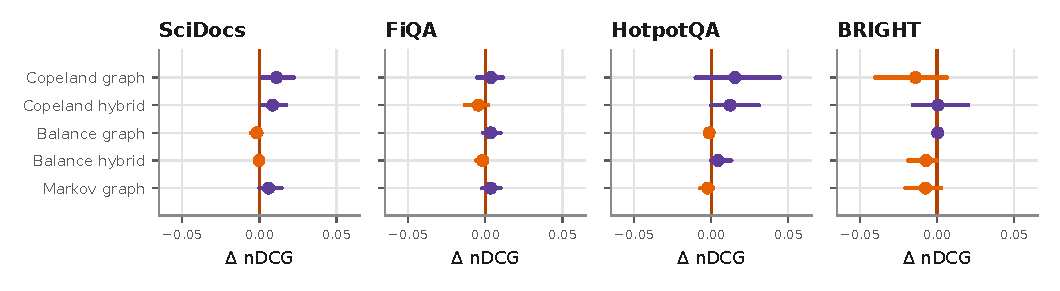
\includegraphics[width=\linewidth,trim=0 0 225 0,clip]{Fig3.pdf}\\[6pt]
\hfill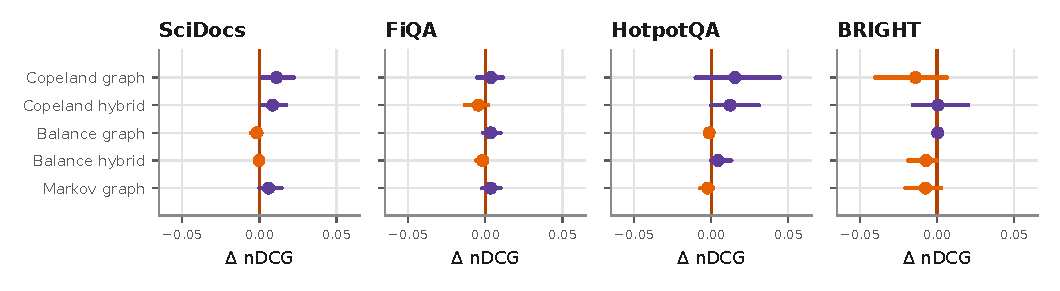
\includegraphics[width=0.789\linewidth,trim=285 0 0 0,clip]{Fig3.pdf}
\caption{Greedy-minus-unrepaired nDCG effects and pointwise 95\% bootstrap intervals under ms1 and candidate-conditioned IDCG: nDCG@20 for SciDocs/FiQA/BRIGHT (120/120/50 queries), nDCG@10 for HotpotQA (52). Purple/orange marks positive/negative point estimates, not significance; the vertical line is zero. Upper panels: SciDocs and FiQA; lower panels: HotpotQA and BRIGHT, with the same method-row order. None of the active family's 20 comparisons survives Holm correction; interval positions are not corrected discovery decisions}
\label{fig:forest}
\end{figure*}


\section{Structural and Ranking Sensitivity}\label{sec:si-structural}
\subsection{Canonical construction and cost}
Figures~\ref{fig:si-scale} and~\ref{fig:si-cycles} show source-scale sensitivity and cyclicity. Conditional BM25 edge-weight share is 0.988 raw/0.512 normalized. Normalization changes source influence; it does not establish calibrated correctness. Construction-time mutual dropping and post-hoc reciprocal deletion remain different interventions, with the SciDocs 11.7\% versus 10.8\% residual cyclicity distinction retained.
\begin{figure}[tp]\centering
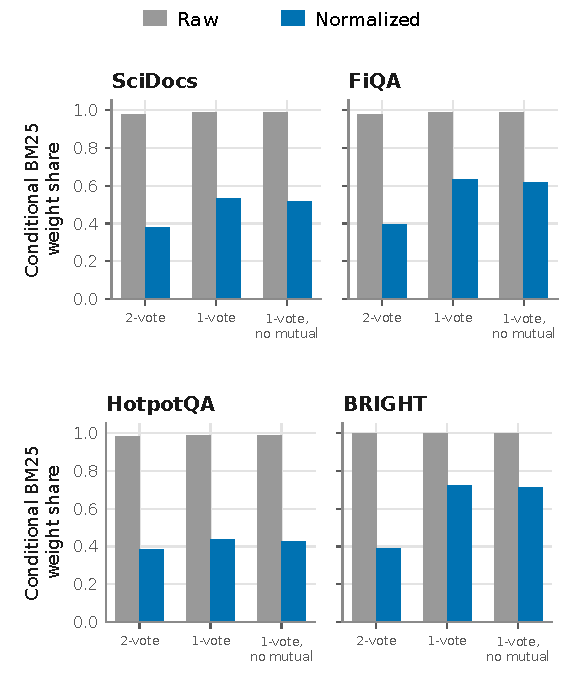
\includegraphics[width=\linewidth]{ESM_Fig1.pdf}
\caption{Source-scale sensitivity on the fixed canonical cohorts (120 SciDocs, 120 FiQA, 52 HotpotQA and 50 BRIGHT queries). Within each dataset/regime, conditional share is the ratio of summed BM25 weight to summed total source weight over retained directed-edge support with positive BM25 contribution. Gray/blue bars use raw/normalized margins. Panels preserve the original plotted values; 2-vote, 1-vote and 1-vote no mutual denote ms2, ms1 and construction-time mutual dropping}
\label{fig:si-scale}\end{figure}
\begin{figure}[htbp]\centering
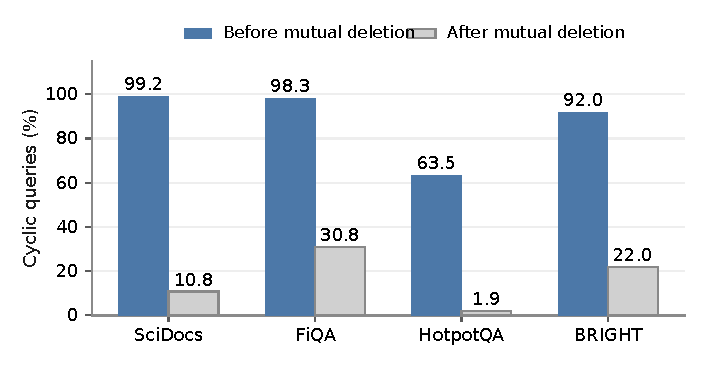
\includegraphics[width=\linewidth]{ESM_Fig2.pdf}
\caption{Cyclic-query percentages under ms1 before and after post-hoc reciprocal-edge deletion (120 SciDocs, 120 FiQA, 52 HotpotQA and 50 BRIGHT queries). This post-hoc diagnostic is distinct from construction-time mutual dropping}
\label{fig:si-cycles}\end{figure}

Tables~\ref{tab:si-cycles} and~\ref{tab:exact-vs-greedy} retain canonical cycle rates and deletion costs, respectively.
\begin{supplementtable}\caption{Canonical structural rates. FAS fraction is the mean within-graph ratio of greedy-deleted weight to original total edge weight (zero for zero-weight graphs); displayed zeros may hide small positive values}\label{tab:si-cycles}\papertable
\begin{tabularx}{\linewidth}{@{}lYrrr@{}}\toprule
Dataset&Regime&Cyclic\%&Post-mutual\%&FAS fraction\\\midrule
SciDocs&ms2&0.0&0.0&0.000\\
&ms1&99.2&10.8&0.074\\
&ms1\_drop\_mutual&11.7&11.7&0.002\\\addlinespace
FiQA&ms2&0.0&0.0&0.000\\
&ms1&98.3&30.8&0.080\\
&ms1\_drop\_mutual&30.8&30.8&0.004\\\addlinespace
HotpotQA&ms2&0.0&0.0&0.000\\
&ms1&63.5&1.9&0.029\\
&ms1\_drop\_mutual&1.9&1.9&0.000\\\addlinespace
BRIGHT&ms2&0.0&0.0&0.000\\
&ms1&92.0&22.0&0.055\\
&ms1\_drop\_mutual&22.0&22.0&0.003\\\bottomrule
\end{tabularx}\end{supplementtable}
\begin{supplementtable}
  \caption{Structural gap on cyclic instances ($n=379$, pooled regimes):
    mean feedback-arc weight removed by exact versus greedy repair.
    Relative reduction is from greedy to exact. Retrieval-level
    exact-versus-greedy and exact-versus-unrepaired Holm outcomes appear
    in the accompanying text (all nonsignificant after correction).}
  \label{tab:exact-vs-greedy}
  \sncstable
  \begin{tabular}{@{}lrrr@{}}
    \toprule
    Dataset & Wt.\ removed (exact) & Wt.\ removed (greedy) & Reduction \\
    \midrule
    SciDocs  & $6.14$ & $8.19$ & $25.1\%$ \\
    \addlinespace
    FiQA     & $4.51$ & $6.37$ & $29.2\%$ \\
    \addlinespace
    HotpotQA & $1.55$ & $1.80$ & $13.4\%$ \\
    \addlinespace
    BRIGHT   & $3.07$ & $3.95$ & $22.3\%$ \\
    \bottomrule
  \end{tabular}
\end{supplementtable}
On the 379 cyclic query--regime records, greedy/exact deletion sets differ in 87.9\%, and 333 have strictly lower exact deletion cost. The average recorded deletion weights are 6.24 greedy/4.60 exact, a 26.3\% mean reduction. These structural comparisons do not identify the sign of retrieval effects.

\subsection{Prospective construction variants}
All 200 model/query/construction graphs reuse 20 identities. Qwen's two symmetric variants coincide, as do Smol's strict and symmetric-both-valid graphs. Every cyclic graph has saved nonempty deletions and a repaired DAG. Tables~\ref{tab:si-construction} and~\ref{tab:construction-utility} report the full structural and utility matrices; Table~\ref{tab:construction-domains} separates domains. Figure~\ref{fig:si-opportunities} summarizes the repeated opportunity counts. No rule is selected by test relevance.
\begingroup\renewcommand{\sncstable}{\papertable\renewcommand{\arraystretch}{1.25}}
\begin{supplementtable}\caption{Graph-construction sensitivity. E = retained edges; C = cyclic graphs; T = cyclic triads; SCC = maximum strongly connected component size; deletion and full-ranking change counts are G/E (greedy/exact). Q/S denote Qwen/Smol. A cyclic triad is a directed three-node cycle; a strongly connected component is a maximal mutually reachable node set. All counts cover twenty queries per row.}\label{tab:si-construction}
\sncstable
\begin{tabularx}{\linewidth}{@{}lYrrrrrr@{}}\toprule
Model & Rule & E & C & T & SCC & Deleted & Rank changes \\\midrule
Q & Strict & 289 & 0 & 0 & 1 & 0/0 & 0/0 \\
Q & AB & 728 & 8 & 37 & 9 & 33/16 & 8/8 \\
Q & BA & 656 & 8 & 46 & 12 & 55/18 & 7/6 \\
Q & Sym. both & 665 & 5 & 5 & 6 & 8/5 & 4/4 \\
Q & Sym. avail. & 665 & 5 & 5 & 6 & 8/5 & 4/4 \\
S & Strict & 144 & 1 & 1 & 3 & 1/1 & 1/1 \\
S & AB & 1250 & 13 & 108 & 12 & 133/38 & 13/12 \\
S & BA & 1253 & 12 & 212 & 12 & 82/58 & 11/11 \\
S & Sym. both & 144 & 1 & 1 & 3 & 1/1 & 1/1 \\
S & Sym. avail. & 257 & 5 & 11 & 10 & 14/8 & 5/5 \\
\bottomrule\end{tabularx}\end{supplementtable}
\begin{supplementtable}
\caption{Exploratory sensitivity on the same $20$ independent queries per model. Cyc = cyclic graphs; Opp = cyclic graphs with at least one judged-positive candidate; U/G/E = unrepaired/greedy/exact nDCG@10. Qwen's two symmetric variants coincide. No alternative becomes a new primary protocol.}
\label{tab:construction-utility}
\sncstable
\begin{tabularx}{\linewidth}{@{}lYrrrrr@{}}
\toprule
Model & Construction & Cyc & Opp & U & G & E \\
\midrule
Qwen & Strict & $0$ & $0$ & $0.126872$ & $0.126872$ & $0.126872$ \\
& AB only & $8$ & $3$ & $0.109908$ & $0.109908$ & $0.109908$ \\
& BA only & $8$ & $4$ & $0.110179$ & $0.109416$ & $0.110179$ \\
& Symmetric (both/available) & $5$ & $2$ & $0.121881$ & $0.121881$ & $0.121881$ \\
\addlinespace
Smol & Strict & $1$ & $0$ & $0.097435$ & $0.097435$ & $0.097435$ \\
& AB only & $13$ & $6$ & $0.105196$ & $0.085103$ & $0.105196$ \\
& BA only & $12$ & $4$ & $0.055740$ & $0.047407$ & $0.051396$ \\
& Symmetric (both valid) & $1$ & $0$ & $0.097435$ & $0.097435$ & $0.097435$ \\
& Symmetric (available) & $5$ & $2$ & $0.088779$ & $0.088779$ & $0.088779$ \\
\bottomrule
\end{tabularx}
\end{supplementtable}\endgroup
\FloatBarrier
\clearpage\begingroup\papertable\renewcommand{\arraystretch}{1.12}\begin{longtable}{@{}llrrrrr@{}}
\caption{Exploratory full-query nDCG@10 by model, construction and dataset. U/G/E/SR = unrepaired/greedy/exact/SpringRank. Opp = cyclic-positive queries. Qwen/Smol identify the models; FiQA/SciD/BR denote FiQA/SciDocs/BRIGHT, with $7/7/6$ queries. All-query variant means are in Table~\ref{tab:construction-utility}.}\label{tab:construction-domains}\\
\toprule Model & Rule/domain & Opp & U & G & E & SR \\\midrule\endfirsthead
\caption[]{Domain-specific construction comparisons (continued)}\\
\toprule Model & Rule/domain & Opp & U & G & E & SR \\\midrule\endhead
Qwen & Strict/FiQA & 0 & $0.2267$ & $0.2267$ & $0.2267$ & $0.2474$ \\
Qwen & Strict/SciD & 0 & $0.0242$ & $0.0242$ & $0.0242$ & $0.0242$ \\
Qwen & Strict/BR & 0 & $0.1301$ & $0.1301$ & $0.1301$ & $0.1301$ \\
\addlinespace[3pt]
Qwen & AB/FiQA & 1 & $0.2267$ & $0.2267$ & $0.2267$ & $0.2226$ \\
Qwen & AB/SciD & 0 & $0.0242$ & $0.0242$ & $0.0242$ & $0.0242$ \\
Qwen & AB/BR & 2 & $0.0736$ & $0.0736$ & $0.0736$ & $0.0736$ \\
\addlinespace[3pt]
Qwen & BA/FiQA & 2 & $0.2051$ & $0.2029$ & $0.2051$ & $0.1706$ \\
Qwen & BA/SciD & 0 & $0.0187$ & $0.0187$ & $0.0187$ & $0.0173$ \\
Qwen & BA/BR & 2 & $0.1061$ & $0.1061$ & $0.1061$ & $0.1061$ \\
\addlinespace[3pt]
Qwen & Sym. both/FiQA & 1 & $0.2180$ & $0.2180$ & $0.2180$ & $0.2226$ \\
Qwen & Sym. both/SciD & 0 & $0.0187$ & $0.0187$ & $0.0187$ & $0.0173$ \\
Qwen & Sym. both/BR & 1 & $0.1301$ & $0.1301$ & $0.1301$ & $0.1301$ \\
\addlinespace[3pt]
Qwen & Sym. avail./FiQA & 1 & $0.2180$ & $0.2180$ & $0.2180$ & $0.2226$ \\
Qwen & Sym. avail./SciD & 0 & $0.0187$ & $0.0187$ & $0.0187$ & $0.0173$ \\
Qwen & Sym. avail./BR & 1 & $0.1301$ & $0.1301$ & $0.1301$ & $0.1301$ \\
\midrule
Smol & Strict/FiQA & 0 & $0.1705$ & $0.1705$ & $0.1705$ & $0.1374$ \\
Smol & Strict/SciD & 0 & $0.0242$ & $0.0242$ & $0.0242$ & $0.0242$ \\
Smol & Strict/BR & 0 & $0.0976$ & $0.0976$ & $0.0976$ & $0.0976$ \\
\addlinespace[3pt]
Smol & AB/FiQA & 4 & $0.2226$ & $0.1788$ & $0.2226$ & $0.1903$ \\
Smol & AB/SciD & 0 & $0.0187$ & $0.0187$ & $0.0187$ & $0.0187$ \\
Smol & AB/BR & 2 & $0.0691$ & $0.0532$ & $0.0691$ & $0.0560$ \\
\addlinespace[3pt]
Smol & BA/FiQA & 2 & $0.0530$ & $0.0498$ & $0.0612$ & $0.0530$ \\
Smol & BA/SciD & 0 & $0.0153$ & $0.0153$ & $0.0153$ & $0.0153$ \\
Smol & BA/BR & 2 & $0.1061$ & $0.0821$ & $0.0821$ & $0.1061$ \\
\addlinespace[3pt]
Smol & Sym. both/FiQA & 0 & $0.1705$ & $0.1705$ & $0.1705$ & $0.1374$ \\
Smol & Sym. both/SciD & 0 & $0.0242$ & $0.0242$ & $0.0242$ & $0.0242$ \\
Smol & Sym. both/BR & 0 & $0.0976$ & $0.0976$ & $0.0976$ & $0.0976$ \\
\addlinespace[3pt]
Smol & Sym. avail./FiQA & 0 & $0.1491$ & $0.1491$ & $0.1491$ & $0.1229$ \\
Smol & Sym. avail./SciD & 0 & $0.0209$ & $0.0209$ & $0.0209$ & $0.0209$ \\
Smol & Sym. avail./BR & 2 & $0.0976$ & $0.0976$ & $0.0976$ & $0.0736$ \\
\bottomrule\end{longtable}\endgroup
\begin{figure}[tp]\centering
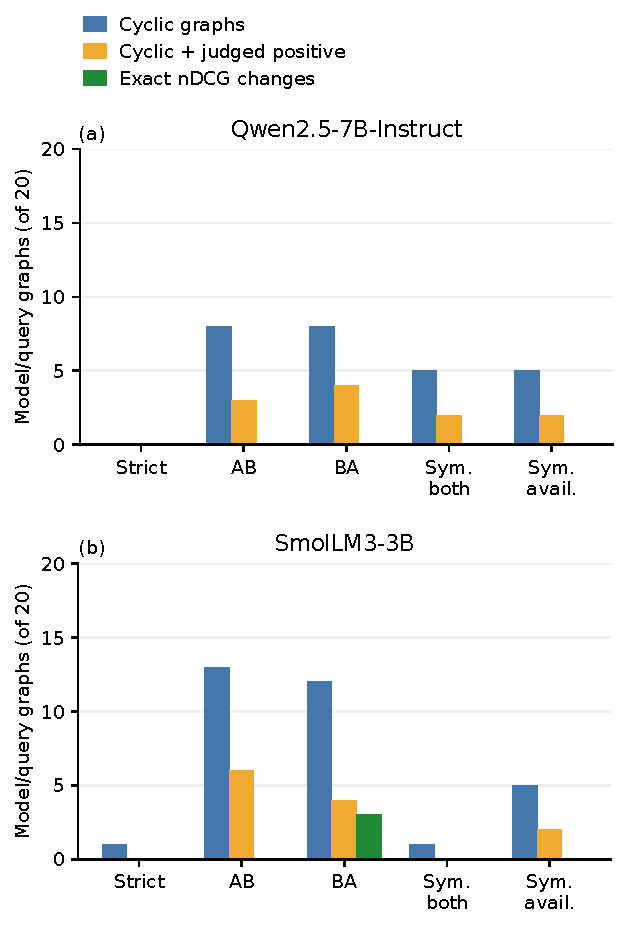
\includegraphics[width=0.88\linewidth]{ESM_Fig3.pdf}
\caption{Exploratory opportunity counts on the same 20 query identities across all five rules, separately for (a) Qwen2.5-7B-Instruct and (b) SmolLM3-3B. Blue counts cyclic graphs, orange cyclic graphs containing a judged-positive candidate, and green nonzero exact-minus-unrepaired full-query nDCG@10 records. Counts are descriptive repeated views; cyclic-positive eligibility alone does not imply utility improvement}
\label{fig:si-opportunities}\end{figure}
Model-averaged AB-only greedy effect is −0.010046, pointwise interval [−0.027757,0], raw p=0.5; AB-only exact is zero. BA-only greedy gives−0.004548, interval [−0.012177,−0.000140], raw p=0.125; BA-only exact gives−0.002172, interval [−0.010946,0.004430], raw p=0.75. Both symmetric constructions have zero observed repair effects. All eight Holm p-values are one. Six of nine nonzero branch records change order within a fixed top-ten set; these records cover six query identities. Smol BA-only exact improves FiQA 3705, harms BRIGHT biology 57 and FiQA 9349 and ties 17 queries. These are conditional outcome descriptions, not a selection rule.

The judged-positive subset contains seven of 20 prospective pools. Conditional strict Qwen/Smol means are 0.362491/0.278386, compared with principal all-query means 0.126872/0.097435. The 13 zero-positive pools remain in principal estimates. Neither conditioning nor treating unjudged documents as evaluation zero restores missing relevant candidates.

\section{Cached LLM Evidence and Relevance Attribution}\label{sec:si-cached}
\subsection{Primary and selected-cache contracts}
The corrected primary cache uses six independent queries, three SciDocs/three FiQA, eight candidates and four historical provider identities: Azure GPT-4.1-mini, Cohere command-r-plus-08-2024, Fireworks gpt-oss-120b and Gemini2.5Flash. These serving names are historical aliases. Each provider has 168 unordered query--document pairs with both orientations, giving 1,344 responses. Strict parsing yields 1,334 valid directional responses, six invalid responses and four abstentions. Every individual-provider graph is a DAG; all six aggregate graphs are cyclic.

The earlier cluster analysis used a legacy parser that could default invalid output to A and resolve reversal conflicts toward the first input. It also selected the better whole-graph greedy/exact utility using qrels before averaging 20 conditions per query. Its saved difference +0.00019, cluster interval [−0.00072,0.00140], exact p=0.875 concerns that historical estimand, not the corrected aggregate-only replay. Subtracting it from+0.001010 would not isolate a parsing effect. Both use only six independent queries.

Table~\ref{tab:corrected-llm} retains the primary and selected-cache repair effects.
\begin{supplementtable}
  \caption{Exploratory cached-LLM repair effects with fixed Copeland and
    full-query nDCG@10. Primary: six independent queries; pool variants
    reuse them. Selected-cache strata: selected, disjoint provider-availability
    groups. Values are mean repaired-minus-unrepaired differences, not
    effects of changing pools.}
  \label{tab:corrected-llm}
  \sncstable
  \begin{tabularx}{\linewidth}{@{}Yrrr@{}}
    \toprule
    Population / graph & Queries & Greedy $\Delta$ & SCIP $\Delta$ \\
    \midrule
    Primary pool 8, four-provider & 6 & $+0.001010$ & $+0.001010$ \\
    Complete pool 6, four-provider & 6 & $+0.001732$ & $+0.001732$ \\
    Sparse pool 8, four-provider & 6 & $-0.003920$ & $-0.004930$ \\
    Sparse pool 10, four-provider & 6 & $-0.006396$ & $-0.006396$ \\
    Selected cache, two-provider & 110 & $-0.000950$ & $+0.003164$ \\
    Selected cache, four-provider & 103 & $-0.002248$ & $+0.004840$ \\
    \bottomrule
  \end{tabularx}
\end{supplementtable}
The selected cache contains 213 disjoint-from-primary identities, with two-provider110 and four-provider103 availability strata. Fixed Copeland exact effects are +0.003164, interval [0.000060,0.007053], raw p=0.09449, and+0.004840, interval [−0.001427,0.014088], raw p=0.25627. Both adjusted p-values equal one in their saved exploratory family. Only 18/213 queries have complete matched source-score maps for graph-free fusion. The 217 score-derived task records on these queries are not genuine-LLM observations.

\subsection{Saved-grade attribution and descriptive cases}
The attribution selects the already saved strict-agreement, real-LLM, selected-cache aggregate tasks, with Copeland, empty insertion-order seed and one baseline task per dataset/query. It compares none/greedy/exact permutations from 213 checkpoints, preserving the complete 15-document candidate set. The frozen qrel maps define evaluated top-ten grade vectors; missing labels map to evaluation zero. Saved metric differences use the inherited $10^{-12}$ zero tolerance. The initial descriptive derivation used saved metric differences; the independent recovery check below additionally recomputes discounted gain and nDCG from the frozen permutations and grades.

The original private 426-row attribution table retains dataset/query/unit/task identities, baseline-source CSV line numbers, checkpoint hashes and descriptive classes. Its two repair records per query are dependent. All 74 positive-pool changed-ranking/zero-nDCG cases per repair have the same evaluated top-ten grade sequence. Greedy/exact zero-positive ranking-change counts are 69/61. All-moved-unjudged indicators are 55/58 among the positive-pool equal-profile cases; positive-document movement occurs in 6/5 and explicitly zero-grade movement in 13/11. The movement indicators are not a new population hypothesis test.

For independent reconstruction, all 219 files in the original attribution source manifest still match their hashes: 213 task checkpoints, four frozen qrel maps, the selection-metrics table and the derivation script. A separate standard-library verifier takes complete saved branch permutations, per-candidate grades and explicit-judgment flags, and the full-query ideal grades. It reconstructs moved-document and membership indicators, top-ten grade profiles, nDCG and the mutually exclusive classifications without reading reference classifications first. All 426 branch records and 6,816 reference fields match; maximum numerical difference is $2.22\times10^{-16}$. Query-local integer relabeling preserves the permutations and distinguishes explicit zero grades from unjudged documents. This verifies attribution conditional on saved rankings and labels; it does not regenerate provider comparisons or original repair choices. The recovered input projection remains private pending applicable sharing clearance.

\subsection{Dataset, availability and positive-pool composition}
The new descriptive script reconstructs the same 426 paired branch records before reading reference classifications, then joins original dataset/query identities to saved provider-availability and cyclicity metadata. All 219 original source files are hash-verified. The complete cross-tabulation in Table~\ref{tab:selected-composition-detail} has fixed dataset, two/four-provider and positive-availability axes; empty cells are retained. The two repair branches share 213 identities. No canonical records are added, no favorable cell is selected and no new significance tests are performed.

Across positive-containing pools ($N=134$, 120 cyclic), greedy/exact leave 23/35 rankings unchanged, change 111/99 and change measured utility in 37/25 (15/16 gains and 22/9 harms). The other 74/74 changed rankings retain their evaluated profile. Across zero-positive pools ($N=79$, 71 cyclic), 10/18 rankings are unchanged and 69/61 change without a measured change. There is no changed-profile/zero-metric positive-pool residual under the inherited $10^{-12}$ tolerance. The main composition table gives the overlapping dataset and availability marginals.

The zero-positive subset is 36 SciDocs, 38 FiQA, four BRIGHT and one HotpotQA. Positive-pool fixed-profile zeros occur in all four datasets and both strata. The HotpotQA/two-provider/zero-positive cell is empty; HotpotQA/four-provider/zero-positive has one query and both BRIGHT zero-positive cells have two. These are sparse descriptive counts, not reliable estimates of subgroup efficacy. Availability is observational and confounded with datasets and evidence retention. Judged-positive absence is not true irrelevance.
\begin{supplementtable}\papertable\setlength{\tabcolsep}{3pt}
\caption{Complete dataset $\times$ provider-availability $\times$ judged-positive-availability decomposition. $P+$ is yes/no positive pool; $C$ counts cyclic graphs (cyclic-positive cases in yes rows). Same/changed count full rankings; Equal counts changed rankings with identical evaluated grade profiles, including zero-positive cases. The last six columns contain paired greedy/exact counts. Empty cells have $N=0$; they are not estimates of population behavior.}\label{tab:selected-composition-detail}
\begin{tabular}{@{}lllrrrrrrrr@{}}\toprule
Dataset & Prov. & $P+$ & $N$ & $C$ & Same & Changed & Equal & $\Delta U$ & Gain & Harm\\\midrule
SciDocs & 2 & no & 18 & 15 & 4/6 & 14/12 & 14/12 & 0/0 & 0/0 & 0/0\\
SciDocs & 2 & yes & 23 & 21 & 5/8 & 18/15 & 7/9 & 11/6 & 4/4 & 7/2\\
SciDocs & 4 & no & 18 & 18 & 0/0 & 18/18 & 18/18 & 0/0 & 0/0 & 0/0\\
SciDocs & 4 & yes & 18 & 18 & 1/1 & 17/17 & 9/14 & 8/3 & 3/3 & 5/0\\
\addlinespace[3pt]
FiQA & 2 & no & 19 & 17 & 3/8 & 16/11 & 16/11 & 0/0 & 0/0 & 0/0\\
FiQA & 2 & yes & 22 & 21 & 3/8 & 19/14 & 13/10 & 6/4 & 3/1 & 3/3\\
FiQA & 4 & no & 19 & 19 & 0/1 & 19/18 & 19/18 & 0/0 & 0/0 & 0/0\\
FiQA & 4 & yes & 16 & 16 & 0/1 & 16/15 & 14/12 & 2/3 & 2/3 & 0/0\\
\addlinespace[3pt]
BRIGHT & 2 & no & 2 & 0 & 2/2 & 0/0 & 0/0 & 0/0 & 0/0 & 0/0\\
BRIGHT & 2 & yes & 18 & 8 & 11/14 & 7/4 & 5/3 & 2/1 & 1/1 & 1/0\\
BRIGHT & 4 & no & 2 & 2 & 0/0 & 2/2 & 2/2 & 0/0 & 0/0 & 0/0\\
BRIGHT & 4 & yes & 20 & 20 & 1/0 & 19/20 & 13/15 & 6/5 & 1/2 & 5/3\\
\addlinespace[3pt]
HotpotQA & 2 & no & 0 & 0 & 0/0 & 0/0 & 0/0 & 0/0 & 0/0 & 0/0\\
HotpotQA & 2 & yes & 8 & 7 & 2/3 & 6/5 & 6/4 & 0/1 & 0/1 & 0/0\\
HotpotQA & 4 & no & 1 & 0 & 1/1 & 0/0 & 0/0 & 0/0 & 0/0 & 0/0\\
HotpotQA & 4 & yes & 9 & 9 & 0/0 & 9/9 & 7/7 & 2/2 & 1/1 & 1/1\\
\bottomrule\end{tabular}\end{supplementtable}

The main-paper observed case C1 is selected deterministically among greedy positive-pool equal-profile cases with only unjudged movement affecting the top ten: minimize the number of moved positions, then sort dataset/query identity. The identity, full source linkage and private row-level outputs remain in the restricted study archive. Only the derived BRIGHT two-provider case narrative (ranks 2/5, fixed grade prefix and utility) is shown; no raw benchmark material or provider response is published. This illustration is not a new independent observation or an optimum envelope.

All four symmetric-available cyclic-positive cells are shown in Table~\ref{tab:si-cases}. They contain only three independent query identities. Each has one judged-positive candidate. Every moved document is unjudged and no judged-positive position changes. Exact top-ten membership is unchanged in all four; greedy Qwen/FiQA 7284 changes membership without utility. These are returned-solution cases, not certified complete optimum sets.
\begin{supplementtable}\caption{Four descriptive cyclic-positive model/query cells on three queries. G/E denote greedy/exact; moved documents are all unjudged}\label{tab:si-cases}\papertable
\begin{tabularx}{\linewidth}{@{}Yrrl@{}}\toprule
Model / query&Deleted G/E&Moved G/E&Top10 set G/E\\\midrule
Qwen / BRIGHT biology 61&2/1&2/4&No/No\\
Qwen / FiQA 7284&3/1&7/2&Yes/No\\
Smol / BRIGHT biology 61&5/2&6/4&No/No\\
Smol / BRIGHT biology 57&1/1&2/3&No/No\\\bottomrule
\end{tabularx}\end{supplementtable}

Saved structural--utility associations are heterogeneous: exact removed-weight/effect Spearman association is +0.3094 for the Azure selected-cache graphs, but−0.0441/−0.0682 for the two aggregate strata. These are descriptive existing associations without predictive-generalization claims. Removed weight measures intervention magnitude, not necessarily better optimization. Neither a global absence of association nor a causal relationship follows.

\section{External Controls and Candidate Coverage}\label{sec:si-controls}
\subsection{Matched graph and trained relevance controls}
The original-graph SpringRank comparison preserves exact candidates, directed weights and full-query qrels, including isolates. The six-query primary mean 0.882760 ties both selected repairs query by query. On 213 selected queries, means are 0.357436 SpringRank,0.353838 unrepaired,0.352261 greedy,0.357813 exact and 0.352890 Bradley--Terry-style aggregation. Exact versus SpringRank has 23 wins,12 losses and 178 ties. All 79 zero-positive pools remain; the 134 positive-containing subset has means 0.568163/0.568763 for SpringRank/exact. These are coverage-conditioned descriptions, not improved candidate recall.
Table~\ref{tab:springrank} provides all saved matched SpringRank contrasts.
\begin{supplementtable}
  \caption{Exploratory original-graph SpringRank comparison, primary
    $\lambda=0$, full-query nDCG@10. U/G/E are unrepaired/greedy/exact
    Copeland. Positive $\Delta$ favors SpringRank; intervals are pointwise
    paired query-bootstrap 95\% intervals. Holm covers these eight tests.
    Selected denotes the 213-query cache. Six-query comparisons with G/E tie on every query; displayed zeros
    suppress floating-point errors below $10^{-12}$.}
  \label{tab:springrank}
  \sncstable
  \begin{tabularx}{\linewidth}{@{}L{2.05cm}Yrrr@{}}
    \toprule
    Cohort & Control & $\Delta$ & 95\% interval & Holm $p$ \\
    \midrule
    Six ($n=6$) & U-Copeland & $+0.001010$ & $[0,0.003030]$ & 1 \\
     & G-Copeland & $0$ & $[0,0]$ & 1 \\
     & E-Copeland & $0$ & $[0,0]$ & 1 \\
     & Bradley--Terry & $+0.001010$ & $[0,0.003030]$ & 1 \\
    \midrule
    Selected ($n=213$) & U-Copeland & $+0.003598$ & $[-0.003052,0.011223]$ & 1 \\
     & G-Copeland & $+0.005175$ & $[-0.000692,0.012694]$ & 1 \\
     & E-Copeland & $-0.000377$ & $[-0.006577,0.006980]$ & 1 \\
     & Bradley--Terry & $+0.004546$ & $[-0.000582,0.010750]$ & 1 \\
    \bottomrule
  \end{tabularx}
\end{supplementtable}

The adapted PRP-Graph pilot uses frozen 20-document pools, pinned FLAN-T5-large and the published implementation's probability-aware comparison/Swiss acquisition and personalized PageRank logic \cite{luo2024prpgraph}. Runtime adapters call unchanged modules directly where the public command-line round handling is unsuitable; no test-qrel interpolation is tuned. Its published TREC-COVID run, original first-stage index and recorded graph are not reproduced. Local changes are documented rather than described as exact reproduction of published effectiveness.

The trained \texttt{BAAI/bge-reranker-v2-m3} cross-encoder follows its official model-card procedure \cite{bge2024modelcard}. It supplies exactly 400 PRP-pool and 240 prospective-pool query--document scores, with 32-bit floating-point (FP32) inference, batch size 8, joint maximum length 512, longest-first/right truncation, raw logits and document-ID ties. These 640 scores are not 640 independent queries. Training and compute differ from the generative models. Table~\ref{tab:external-controls} preserves the full absolute means, including PageRank.
\begin{supplementtable}
\caption{Matched full-query nDCG@10. Each column uses $20$ independent queries. U/G/E = unrepaired/greedy/exact Copeland; SR = SpringRank; BT = Bradley--Terry. Shared BM25/BGE values in the prospective columns are one observation per query, not model replications. PRP-native graph methods use its Swiss observations; prospective methods use the strict primary graph, fixed before its repair evaluation.}
\label{tab:external-controls}
\sncstable
\begin{tabularx}{\linewidth}{@{}Yrrr@{}}
\toprule
Method & PRP pilot & Prospective Qwen & Prospective Smol \\
\midrule
BM25 & $0.278865$ & $0.080112$ & $0.080112$ \\
BGE cross-encoder & $0.354547$ & $0.108610$ & $0.108610$ \\
Adapted PRP-Graph & $0.270215$ & --- & --- \\
Unrepaired Copeland & $0.271771$ & $0.126872$ & $0.097435$ \\
Greedy repair & $0.271771$ & $0.126872$ & $0.097435$ \\
SCIP exact repair & $0.271526$ & $0.126872$ & $0.097435$ \\
SpringRank & $0.259999$ & $0.134091$ & $0.085859$ \\
PageRank & $0.232208$ & $0.126872$ & $0.105153$ \\
Bradley--Terry & $0.254006$ & $0.134091$ & $0.089653$ \\
\bottomrule
\end{tabularx}
\end{supplementtable}
On the adapted PRP 20-query cohort, all eight original comparisons against four native Swiss/four random-acquisition controls have Holm p=1. BGE differences and intervals are exploratory pointwise comparisons, not an added confirmatory family. Graph-free canonical macros in Table~\ref{tab:retrieval-holm} similarly provide context rather than paired superiority evidence.

\subsection{Qrels-blind candidate intervention}
Twenty further queries exclude prior newer-cohort identities and exact query-text duplicates. Both arms are frozen before qrels: BM25 top12, versus BGE top12 selected from the same BM25 top100. Retrieval uses unchanged lowercase-alphanumeric BM25, $k_1=1.5$, $b=0.75$, original IDs, title--newline--body text and deterministic document-ID ties. The oracle orders available candidates by qrel gain with full-query IDCG; it is a label-informed ceiling, not achieved reranker effectiveness.
Table~\ref{tab:candidate-intervention} separates overall and dataset-specific candidate coverage.
\begin{supplementtable}
\caption{Candidate intervention: frozen BM25 top-$12$ (A) versus BGE-selected top-$12$ from BM25 top-$100$ (B). Coverage counts pools with judged-positive documents; oracle ceilings use the full-query ideal. Both arms were frozen before qrels access.}
\label{tab:candidate-intervention}
\sncstable
\begin{tabularx}{\linewidth}{@{}Yrrrr@{}}
\toprule
Dataset ($n$) & Coverage A/B & Positive docs A/B & Oracle A & Oracle B \\
\midrule
FiQA ($7$) & $2/4$ & $2/4$ & $0.230450$ & $0.364529$ \\
SciDocs ($7$) & $4/3$ & $5/5$ & $0.224375$ & $0.200150$ \\
BRIGHT biology ($6$) & $0/1$ & $0/1$ & $0.000000$ & $0.102191$ \\
All ($20$) & $6/8$ & $7/10$ & $0.159189$ & $0.228295$ \\
\bottomrule
\end{tabularx}
\end{supplementtable}
Coverage rises 6→8/20, difference +0.10 with interval [−0.10,0.30]. Mean candidate recall rises 0.125000→0.183333 and oracle nDCG 0.159189→0.228295, difference +0.069106 with interval [−0.016958,0.164250], four improvements, one harm and 15 ties. SciDocs loses one positive-containing pool. Of 240 candidates per arm,233 BM25/230 BGE are unjudged. BM25 top100 has positive coverage11/20 and oracle 0.318911; that is a diagnostic ceiling, not a third tuned arm. The inspected relevance labels are not an untouched method-selection set.

\section{Measurement Validity and Prompt Development}\label{sec:si-validity}
\subsection{Prospective reliability and missing controls}
The original JSON prompt includes an A/high illustrative response. It is a plausible source of positional sensitivity, not an isolated cause established by the collection. Qwen has 2,920 valid pairwise outputs with 1,378 abstentions; Smol has 2,772 valid of 2,920, with 148 invalid, all token-capped. Invalidity and capping overlap rather than add. Initial opposite-winner/abstention and repeat denominators are retained in Table~\ref{tab:reliability-detail}. A repeated positional preference can be stable without being correct.
\begin{supplementtable}
\caption{Prospective reliability denominators, separately by model. Pairwise totals include independent repeats; initial orientation denominators exclude repeats. A/B denote the first/second displayed document; AB/BA reverse their presentation and restore actual document identity. Displayed-A rates condition on valid directional observations. Invalid and capped counts overlap; valid abstentions remain separate from invalid or missing responses.}
\label{tab:reliability-detail}\sncstable
\begin{tabularx}{\linewidth}{@{}Yrr@{}}\toprule
Endpoint & Qwen & Smol \\\midrule
Pairwise valid / attempted & $2920/2920$ & $2772/2920$ \\
Valid abstentions & $1378$ & $0$ \\
Directional A / valid directional & $747/1542$ & $2591/2772$ \\
Initial AB/BA discordance / comparable & $591/1320$ & $1051/1195$ \\
Initial opposite-direction winners & $215$ & $1051$ \\
Initial one-abstention pairs & $376$ & $0$ \\
Initial both-abstention pairs & $440$ & $0$ \\
Initial pairs with invalid response(s) & $0$ & $125$ \\
Initial single-invalid / double-invalid pairs & $0/0$ & $113/12$ \\
Invalid pairwise outputs / capped invalid & $0/0$ & $148/148$ \\
Repeat disagreement / comparable & $22/280$ & $14/262$ \\
Repeat comparisons involving invalidity & $0$ & $18$ \\
Valid listwise / attempted & $0/20$ & $10/20$ \\\bottomrule
\end{tabularx}
\end{supplementtable}
Qwen abstentions comprise 1,376 insufficient-information and two ties. Smol invalid pairwise outputs comprise 137 first observations and 11 repeats; initial pairs include 113 single-invalid and 12 double-invalid cases. The 30 invalid listwise outputs terminate normally but are non-JSON, unlike the capped pairwise failures. Missing listwise rankings are never assigned zero utility.

\subsection{Unsuccessful neutral-schema development}
Thirty deterministic repeated pairs across the same 20 development queries, ten pairs per dataset, yield 240 historical controls and 240 neutral-schema responses from two models, two orientations and two independently executed replicates. Only the A/high example is replaced; other rendered text, model settings, truncation, temperature, top-$p$, output cap and per-observation seeds are matched. Controls are historical, not contemporaneously randomized; numerical/hardware effects are not fully excluded.
Table~\ref{tab:si-prompt} retains the descriptive prompt-validity counts.
\begin{supplementtable}
\caption{Prompt-validity development: descriptive pooled counts. Original/neutral prompts share exact pair provenance; neither responses nor pairs are independent queries. A/B denote first/second displayed documents and AB/BA their two orientations. A rate conditions on valid directional outputs; the neutral Smol denominator is only two. ``Corroborated'' requires valid AB/BA choices for the same actual document, with all sixty pair/replicate cases in the denominator. Capping and invalidity overlap; abstentions are valid responses, distinct from missing or invalid outputs.}
\label{tab:si-prompt}
\sncstable
\begin{tabularx}{\linewidth}{@{}lYrrrr@{}}\toprule
Model & Prompt & Valid & Capped & A/directional & Corroborated \\\midrule
Qwen & Original & $120/120$ & $0$ & $40/75$ & $13/60$ \\
& Neutral & $120/120$ & $0$ & $16/40$ & $13/60$ \\
Smol & Original & $119/120$ & $1$ & $114/119$ & $5/60$ \\
& Neutral & $3/120$ & $74$ & $1/2$ & $0/60$ \\\bottomrule
\end{tabularx}
\end{supplementtable}
Qwen abstentions rise 45→80/120. Orientation disagreement falls 36→11/60 while both-abstention rises 11→36 and corroborated directional cases remain 13/60. The primary query-averaged usable-direction difference is zero, interval [−0.1625,0.1750], Holm p=1. Secondary abstention difference is +0.29375, interval [0.19375,0.40000]. Conditional displayed-A change uses 11 defined query cells and is not unconditional debiasing.

Smol neutral outputs contain 117 invalid responses:74 capped and 43 invalid despite normal termination. Of three valid outputs, one abstains. The primary usable-direction difference is −0.0875, interval [−0.2000,0], Holm p=0.5; secondary validity difference is −0.96875, interval [−0.99375,−0.93750]. All neutral orientation/repeat cases involve invalidity, so no repeat-disagreement rate is estimable. Qwen repeat disagreement changes 4→2/60; Smol original is 1/59 and neutral unavailable, not zero. Two surviving neutral Smol directional responses do not validate debiasing.

Primary inference weights 20 query means equally, separately by model, with Holm over two corroboration contrasts. Secondary intervals are pointwise. The frozen code derives endpoint/model seeds from root 20261025; literal-root sensitivity leaves Qwen's primary interval unchanged and changes Smol's lower endpoint to −0.2125. This disclosed seed-prose ambiguity does not replace the frozen implementation result. The unsuccessful variant neither revises primary retrieval inference nor validates a better instrument.

\section{Related-Work and Reuse Detail}\label{sec:si-related}
The published acyclic-ranking pipeline concerns graph disagreement and ranking recovery; pruning, exact add-back, min-cut exchange and ranking--MWFAS theory remain prior work \cite{vahidi2026acyclicranking}. The present audit estimates deletion effects against external retrieval qrels. Related graph-benchmark work studies graph identity and structural algorithm comparisons; its benchmark resources and numerical outcomes are not presented as new retrieval data. An identified related-manuscript/status comparison is prepared separately for confidential editorial disclosure; its delivery is pending.

PRP-Graph evaluates probability-aware graph reranking \cite{luo2024prpgraph}; direct SpringRank estimates hierarchy on original graphs \cite{debacco2018springrank}. These are different interventions from fixed-extractor edge deletion. Pairwise prompting and listwise prompting have established effectiveness evidence under their own evaluation contracts \cite{qin-etal-2024-large,sun-etal-2023-chatgpt}; the present qualified null does not refute those results. Nor does a graph-internal disagreement optimum imply external nDCG optimality.

\subsection{Version-specific public-preprint comparison}
The public Research Square v1 preprint (posted 17 June 2026) already reports the construction/repair/extraction distinction and conditional retrieval effects \cite{vahidi2026retrievalpreprint}. Those are not newly discovered claims. Table~\ref{tab:preprint-delta} distinguishes reused evidence from the present explanatory increment. It is a version-specific content map, not a claim that all differences are independent new experiments.
\begin{supplementtable}
\caption{Public preprint v1 versus this JDSA revision: contribution boundaries. Section/table pointers in the middle column refer to the preprint. Reused observations are not independent replications.}\label{tab:preprint-delta}\papertable
\begin{tabularx}{\linewidth}{@{}L{2.4cm}L{3.5cm}Y@{}}\toprule
Component & Already present in v1 & Current scope / difference\\\midrule
Algorithms and theory & Repair/extraction pipeline, established graph formulations & Used as controls; no new algorithm or ranking--MWFAS theorem\\\addlinespace
Benchmarks / records & Four datasets, regime names and stored-score evidence (Sections 4--5) & Reused; cohort and normalization contracts explicit; previously released resources not new datasets\\\addlinespace
Construction & Raw-margin/fixed-threshold legacy results (Section 5.2, Table 6) & Current min--max / retention-matched pipeline; version bridge incomplete; see text\\\addlinespace
Broad retrieval message & Structural gains, conditional retrieval effects (abstract, discussion) & Retained and narrowed; broad consistency/utility distinction is not new\\\addlinespace
Statistical analysis & Earlier saved comparison summaries & Query-block correction preserves effects and 35-test family; original row-independent significance interpretations superseded\\\addlinespace
Opportunity composition & No complete selected-cache branch decomposition & 213 queries / 426 dependent branches locate ranking/profile/utility activity; fixed dataset, availability and positive-pool strata\\\addlinespace
Relevance attribution & No complete saved-profile accounting & 74 positive-pool fixed-profile cases per repair; observed case and all gains/harms retained; identity alone not novelty\\\addlinespace
Exact-optimum choice & A returned optimum does not enumerate all optima & Complete six-graph/eight-repair envelope; one graph utility-varying; finite diagnostic only\\\addlinespace
Reproducibility & Earlier source/results provenance & Independent processed-statistic, profile and finite-envelope checks; input access and historical pins remain limited\\\bottomrule
\end{tabularx}
\end{supplementtable}

The legacy saved publication table exactly matches the preprint's permissive SciDocs/BRIGHT cyclicity summaries, 87.5\%/60.0\%. It is explicitly marked superseded by the later calibrated pipeline. The current primary per-query/ranker min--max and retention-matched construction reports 99.2\%/92.0\%. Both versions retain 120 SciDocs and 50 BRIGHT query counts, but equal counts do not establish identical execution inputs or candidate pools.

Importantly, the current pipeline's raw/fixed reference already reports 97.5\%/88.0\%, rather than the legacy 87.5\%/60.0\%. Its transition to the current primary construction therefore cannot explain the whole historical difference by normalization alone. The legacy script records raw-margin voting and fixed support/margin rules; current manifests record per-query/ranker normalization and dataset/ranker quantile vote thresholds, with aggregate thresholds matching raw retained-edge counts. Calibration uses the evaluated query list without qrel tuning. These establish a pipeline/version and documented construction-contract change, not an isolated causal effect of normalization between legacy and current tables. The exact legacy execution-to-pool/input bridge is not fully reconstructed and remains a disclosed reproducibility limit. Current score/qrel hash matches do not fill that legacy gap.

The current protocol's paired normalization/threshold ablations are the appropriate within-pipeline contrasts. The 87.5\%/60.0\% values are historical context, not a second measurement of the current graphs or evidence of contradictory outcomes under identical conditions. The provenance record names the saved legacy/current tables and exact source hashes. Corrected query-block inference supersedes row-independent significance interpretations while preserving its effect estimand and 35-comparison family. It does not convert reused benchmark observations into new independent evidence.

The separate related MWFAS submission is handled through the existing confidential comparison. A prepared manuscript file has been inspected, but its identity with the actual portal-uploaded version is unverified. No assertion of exact submitted-file identity or cleared overlap is made. A private revision addendum records this uncertainty; confidential identifiers and correspondence are not included in these sources.


Historical selector/headroom work is context rather than a fourth independent test of impossibility. A 419-query mixed-protocol summary over 122,203 dependent rows has preserve/repair/oracle means 0.481487/0.479852/0.483994 and query-level headroom 0.002507824, saved interval [0.002041054,0.003018928]. Benefit/harm/exact-neutral proportions are 28.2/27.2/44.6\%. These meta-averages are not an untouched homogeneous efficacy study. Dependent-row feature p-values do not establish query-level predictability, and the mixed headroom cannot be compared with a canonical MDE as a practical-importance bound. Executed selector failures and mixed-protocol headroom do not establish predictive impossibility; other aggregation/stopping studies address distinct interventions.

\paragraph{Review access and limitations.}
The final reviewer ZIP (35 files; approximately 2.09\,MiB; SHA-256 \texttt{\seqsplit{c31fff08567d3fc0504e0a303a2328067175b8820541746588c30cfee484f7b3}}) provides processed observations, graphs, configurations, saved results and code. Anonymity/offline checks passed. All 35 corrected comparisons independently reproduce at Level~2, confirming 342/290 query populations and zero Holm rejections. Direct checks cover 1,025 graphs (646 acyclic, 379 cyclic) and saved greedy feasibility/cost; other families and exact statuses entail preserved-output checks. Original retrieval scoring is not fully reconstructed. Attribution and the finite six-graph envelope are now independently reconstructed locally from authentic frozen processed inputs, as detailed above; those input projections, original qrels, permutations and provider responses remain excluded from the unchanged 35-file reviewer ZIP. No material rights issue was identified for the included files' proposed confidential review use; the package code has a review-use grant, not an unrestricted public-release license. Confidential delivery requires editorial-channel confirmation; unrestricted public release is not promised.


\subsection{Identified research resources and access limits}
\ifdefined\AnonymousVersion
Author-identifying resource addresses are retained in the identified version and separate editorial records. The private project repository is not a public access method.
\else
The project repository is \url{https://github.com/SoroushVahidi/consistency-aware-llm-rankin}; it remains private pending a history and redistribution audit. The authoritative finalized scientific-source snapshot is commit \texttt{\seqsplit{53083f31a2f698ecc29ba284f8eb7d070567aefd}}. It preserves the corrected source package used for this journal conversion; it is distinct from the earlier implementation foundation \texttt{\seqsplit{c5cfafab73cff427e91fc1fd94aca7cbbae6d5d1}}.

The public derived judgment resource is \href{https://huggingface.co/datasets/SoroushVahidi/consistency-aware-judgments/tree/f9317638ca1cc422661f704168335576d36ca995}{Consistency-Aware Judgments v1 (pinned)}. The recorded license is CC BY-SA 4.0; attribution is Soroush Vahidi. Its four record classes and exclusions are described in Section~S1.4. The related public numerical resource is \href{https://huggingface.co/datasets/SoroushVahidi/ranking-pool-ndcg-results/tree/4d6d9d372c24e541875990923ab5569454b6b44b}{ranking-pool results (pinned)}. Neither resource supplies the missing canonical historical permutations or the recovered private small-instance optimization inputs. Structural resources at \href{https://huggingface.co/datasets/SoroushVahidi/mwfas-heuristic-metrics/tree/5b6cd5620ca0a1c9b3be5e8d996bf8e3c467e79f}{MWFAS heuristic metrics (pinned)} and \href{https://huggingface.co/datasets/SoroushVahidi/mwfas-benchmark-extension/tree/117cd82e5b863238377c5effe7430ce771062cf4}{MWFAS benchmark extension (pinned)} belong to related structural research and are not additional retrieval observations here.
\fi

Authoritative benchmark entry points are \url{https://github.com/allenai/scidocs}, the BEIR FiQA snapshot at \url{https://huggingface.co/datasets/BeIR/fiqa}, \url{https://hotpotqa.github.io/}, and \url{https://huggingface.co/datasets/xlangai/BRIGHT}. Hosted snapshots and license labels do not grant additional rights to underlying source text. The incompletely pinned historical HotpotQA retrieval conversion remains a reproducibility limitation.

External implementations are PRP-Graph at \href{https://github.com/Memelank/PRP-Graph/tree/968e45ee8178f5d3ac44a2b8f11f091af69206d7}{PRP-Graph (pinned source)}, SpringRank at \href{https://github.com/LarremoreLab/SpringRank/tree/f97a489e85e44c553a437e7c6f9e40a800a5ade4}{SpringRank (pinned source)}, and the BGE model card at \href{https://huggingface.co/BAAI/bge-reranker-v2-m3/tree/953dc6f6f85a1b2dbfca4c34a2796e7dde08d41e}{BGE (pinned model card)}. Third-party code is obtained from its source; the SpringRank implementation is not redistributed because of the recorded license inconsistency. These addresses identify resources, not a claim of unrestricted end-to-end reconstruction.


The BEIR corpus snapshots in Table~\ref{tab:si-corpus} have separate qrel repositories: \url{https://huggingface.co/datasets/BeIR/fiqa-qrels} and \url{https://huggingface.co/datasets/BeIR/scidocs-qrels}. Their current public revisions do not establish the versions used historically; frozen qrel hashes remain the comparison anchors. All four original canonical processed qrel files and all 12 BM25/TF-IDF/MiniLM score files remain available privately and match the canonical protocol manifests. Those manifests contain 1,026 query--regime records; the exact study's unchanged 1,025-record roster omits its one historical empty graph. This byte-level recovery does not establish the exact historical corpus conversion or MiniLM weight/tokenizer revision, and no scorer inference is rerun. FiQA's original challenge at \url{https://sites.google.com/view/fiqa/home} specifies noncommercial source-data use. The mirror's license label does not replace that condition, and the paper does not redistribute its text or qrels.

Official checkpoint sources for Table~\ref{tab:si-models} are \href{https://huggingface.co/Qwen/Qwen2.5-7B-Instruct/tree/acbd96531cda22292a3ceaa67e984955d3965282}{Qwen2.5-7B-Instruct (pinned)}, \href{https://huggingface.co/HuggingFaceTB/SmolLM3-3B/tree/a07cc9a04f16550a088caea529712d1d335b0ac1}{SmolLM3-3B (pinned)}, and \href{https://huggingface.co/google/flan-t5-large/tree/0613663d0d48ea86ba8cb3d7a44f0f65dc596a2a}{Flan-T5-large (pinned)}, alongside the BGE card above. The historical MiniLM source is \href{https://huggingface.co/sentence-transformers/all-MiniLM-L6-v2}{MiniLM model card}; its exact historical weight revision has not been recovered. A current model card is not evidence of an immutable historical hosted-provider deployment.

The exact-solver implementations are SCIP, \url{https://github.com/scipopt/scip}, and PySCIPOpt, \url{https://github.com/scipopt/PySCIPOpt} \cite{achterberg2009scip,maher2016pyscipopt}. Recorded canonical versions are SCIP 10.0.2 and PySCIPOpt 6.2.1; current upstream heads are not substituted for those runtime versions. The public PRP-Graph code is Apache 2.0. At the pinned SpringRank revision, the LICENSE file states MIT while \nolinkurl{pyproject.toml} states GPL-3.0-or-later; neither that implementation nor its local runtime adapters are bundled as cleared third-party software.

The public ranking-pool resource validates 93,504 stored measurements, 66 configurations and 1,056 summary rows across 342 query identities. Its standard-library validator checks checksums, schemas and stored means, not the original scoring or this paper's corrected 35-test family. A literal Hub checkout includes an extra \nolinkurl{.gitattributes} transport file outside the release checksum ledger; omit that transport file from a separate verification extraction to run the unmodified validator. Neither this public-output check nor the public judgment resource supplies the recovered private inputs used for the separate attribution and six-graph reconstruction checks.

\bibliography{references}
\end{document}
